\documentclass[UTF8,a4paper,11pt]{ctexart}

\usepackage[margin=1in]{geometry}
\usepackage{amsmath, amssymb}
\usepackage{booktabs}
\usepackage{array}
\usepackage{tabularx}
\usepackage{graphicx}
\usepackage{caption}
\usepackage{subcaption}
\usepackage{float}
\usepackage{hyperref}
\usepackage{xcolor}
\usepackage{enumitem}
\usepackage{setspace}
\usepackage{longtable}

\graphicspath{{report_assets/}}
\captionsetup{font=small, labelfont=bf}
\hypersetup{hidelinks}
\setlist[itemize]{leftmargin=2.0em, itemsep=0.25em, topsep=0.3em}
\setlist[enumerate]{leftmargin=2.2em, itemsep=0.25em, topsep=0.3em}
\setlength{\parindent}{2em}
\setlength{\parskip}{0.2em}
\setstretch{1.15}
\renewcommand{\arraystretch}{1.16}
\emergencystretch=2em
\setlength{\textfloatsep}{8pt plus 2pt minus 2pt}
\setlength{\floatsep}{8pt plus 2pt minus 2pt}
\setlength{\intextsep}{8pt plus 2pt minus 2pt}
\renewcommand{\topfraction}{0.92}
\renewcommand{\bottomfraction}{0.82}
\renewcommand{\textfraction}{0.06}
\renewcommand{\floatpagefraction}{0.78}
\setcounter{topnumber}{5}
\setcounter{bottomnumber}{4}
\setcounter{totalnumber}{8}

\newcommand{\code}[1]{\texttt{\detokenize{#1}}}
\newcommand{\metric}[1]{\texttt{#1}}

\begin{document}

\begin{center}
    {\zihao{1}\bfseries 期末作业\par}
    \vspace{0.5em}
    {\zihao{3}\bfseries 深度学习与空间智能\par}
    \vspace{1.0em}
    {\zihao{2}\bfseries 三维生成与 ACT 空间智能实验报告\par}
    \vspace{0.6em}
    \small
    \begin{tabular}{lll}
        \toprule
        成员 & 学号 & 主要分工 \\
        \midrule
        钱玲萱 & 24110980018 & 题目一物体 A 真实重建与 A/B/C 场景融合 \\
        吉张林 & 25110980010 & 题目一物体 B、C 的 AIGC 三维生成 \\
        朱宇玄 & 25110980033 & 题目二 ACT 实验、结果分析与报告整合 \\
        \bottomrule
    \end{tabular}
\end{center}

\vspace{0.6em}

\begin{center}
    \small
    GitHub 项目地址：\\[-0.1em]
    \url{https://github.com/MayRainStop/3d-generation-act-spatial-intelligence}

    模型权重网盘地址：\\[-0.1em]
    \resizebox{0.88\textwidth}{!}{\url{https://drive.google.com/drive/folders/14n7YY6TVmrlqI1PMlGP65uwwRv75a2do?usp=drive_link}}
\end{center}

\vspace{0.6em}

\begin{abstract}
本文完成题目一三维重建与 AIGC 生成、题目二具身智能模仿学习两部分实验。题目一按照任务顺序依次完成三类物体构建、Mip-NeRF 360 任务场景重建和 A/B/C 场景融合：真实物体 A 以湿巾包为对象，使用 73 张手机多视角图像完成 COLMAP+3DGS 重建；物体 B 使用 threestudio text-to-3D 生成梨形纹理网格；物体 C 使用 Zero123 image-to-3D 从单张红黄水果图生成网格。随后在 \code{garden}、\code{bicycle} 和 \code{counter} 三个场景上使用 COLMAP 稀疏相机与官方 3DGS 流程进行重建，并使用 PSNR、SSIM 和 LPIPS 进行定量评估，其中 \code{counter} 场景主实验取得 PSNR 29.61、SSIM 0.9290、LPIPS 0.1007，\code{garden} 场景主实验取得 PSNR 27.86、SSIM 0.8751、LPIPS 0.1027。最终融合阶段将物体 A、梨形物体 B 和单图生成物体 C 插入重建的 \code{counter} 背景场景并导出 150 帧环绕漫游视频；garden 步数/分辨率消融和 AIGC 路线示例放在题目一主线之后作为附加分析。题目二完成 LeRobot ACT 在 CALVIN 上的跨环境泛化实验，比较 A-only 基础策略和 ABC-mixed 多环境联合策略在未见环境 D 上的 zero-shot 表现；在课程提供的 \code{splitA}/\code{splitB}/\code{splitC}/\code{splitD} 官方划分上，A-only 100000 step 取得 Avg Len 0.855，ABC one-hot、ABC SBERT 和 ABC chunk100 分别取得 0.649、0.787 和 0.696；进一步的 checkpoint sweep 与 seed1 稳健性实验中，ABC SBERT seed1 100000 step 取得 Avg Len 0.923，ABC SBERT seed0 160000 step 取得 0.915；ABC 扩展训练实验在 120000 step checkpoint 取得 Avg Len 1.028。
\end{abstract}

\section{引言}

空间智能任务不仅要求模型理解二维图像内容，还需要恢复或生成三维结构，并进一步在具身交互环境中学习动作策略。本项目包含两个互相关联的方向：一方面，3DGS 和 AIGC 3D 生成关注如何从多视角图像、文本提示或单张图像得到可观察的三维对象与场景；另一方面，LeRobot ACT 关注如何从机器人示范数据中学习动作序列，并在新的 CALVIN 环境中进行 zero-shot 泛化。

本文按任务要求的顺序组织题目一。首先构建三类 3D 对象：真实物体 A 通过手机多视角图像、COLMAP 和 3DGS 重建得到，物体 B 通过 threestudio text-to-3D 生成梨形纹理网格，物体 C 通过 Zero123 image-to-3D 从单张图像生成网格。其次，在 Mip-NeRF 360 的 \code{garden}、\code{bicycle} 和 \code{counter} 场景上训练 3D Gaussian Splatting，并在测试视角上评估图像指标。最后，将 A/B/C 三个物体放入重建的 \code{counter} 背景场景，在 Blender 中统一坐标、材质和相机轨迹并渲染漫游视频。消融实验和额外 AIGC 路线示例集中放在题目一末尾，避免打散主线要求。

LeRobot ACT 部分根据题目要求比较两类策略：仅使用环境 A 数据训练的基础模型，以及混合环境 A、B、C 数据训练的多环境联合模型。为避免用 episode 顺序近似环境标签，本文先用 \code{huiwon/calvin\_task\_ABC\_D} 与 CALVIN 官方 \code{scene\_info} 做严格对齐，随后采用课程提供的 \code{splitA}/\code{splitB}/\code{splitC}/\code{splitD} 显式划分作为最终主结果，并分别构造 A-only 与 ABC-mixed 训练集。


\section{3DGS 与 AIGC 三维生成实验}

\subsection{任务要求与总体路线}

题目一包含三个按顺序衔接的要求。首先，需要构建三类三维对象：物体 A 来自真实物体的手机多视角图像，并通过 COLMAP 与 3D Gaussian Splatting 完成重建；物体 B 来自文本提示，使用 threestudio 的 SDS text-to-3D 路线生成；物体 C 来自单张二维图片，使用 Zero123 类 image-to-3D 路线生成。其次，需要在 Mip-NeRF 360 数据集的 \code{garden}、\code{bicycle} 和 \code{counter} 场景上训练 3DGS，并评估新视角渲染质量。最后，需要将前面得到的 A/B/C 三个物体放入重建场景中，在 Blender 中完成统一坐标、材质和相机轨迹设置，并导出漫游视频。

因此，本节严格按题目要求组织：\S\ref{subsec:task1-objects} 说明物体 A/B/C 的构建，\S\ref{subsec:task1-scenes} 说明 Mip-NeRF 360 场景重建，\S\ref{subsec:task1-fusion} 说明场景融合与视频渲染，\S\ref{subsec:task1-supplement} 再集中放置额外消融和 AIGC 路线示例。实验使用单张 NVIDIA GeForce RTX 4090 D GPU 完成，既支持 3DGS 训练，也支持 threestudio 生成实验。

\begin{table}[!htbp]
    \centering
    \caption{题目一任务要求与本文完成情况对应关系}
    \label{tab:task1-requirement-map}
    \small
    \begin{tabularx}{\textwidth}{lX}
        \toprule
        任务要求 & 本文完成内容 \\
        \midrule
        1. 构建三类 3D 对象 & 物体 A 为湿巾包多视角 COLMAP+3DGS 重建；物体 B 为梨形 text-to-3D 纹理网格；物体 C 为单图 Zero123 路线生成网格 \\
        2. Mip-NeRF 360 场景重建 & 在 \code{garden}、\code{bicycle}、\code{counter} 上训练 3DGS，报告 PSNR、SSIM、LPIPS 和渲染图 \\
        3. A/B/C 与场景融合 & 以 \code{counter} 表面网格为背景，在 Blender 中导入 A/B/C 并导出 150 帧环绕视频 \\
        \bottomrule
    \end{tabularx}
\end{table}

\subsection{物体 A/B/C 的三维构建}
\label{subsec:task1-objects}

物体 A/B/C 分别对应真实重建、文本生成和单图生成三条路线。物体 A 选取一包湿巾作为真实物体，共采集 73 张 800\(\times\)450 手机图像；处理时先执行 COLMAP 特征匹配、稀疏重建和 undistortion，得到 5293 个稀疏三维点，再将 undistorted 图像和 \code{sparse/0} 相机输入 3DGS 训练，训练到 7000 iterations 后导出 146445 个 Gaussian centers。物体 B 使用 threestudio 的 DreamFusion/SDS 配置，由文本 prompt 控制为梨形物体，重点约束 yellow-green skin、red blush、speckles 和 pear silhouette，最终导出梨形纹理网格。物体 C 使用单张红黄渐变水果图片作为输入，通过 Zero123 类新视角约束优化并导出单图生成网格。

\begin{table}[!htbp]
    \centering
    \caption{物体 A/B/C 构建路线与最终资产形态}
    \label{tab:task1-objects}
    \small
    \begin{tabularx}{\textwidth}{lXX}
        \toprule
        物体 & 构建方法 & 最终形态 \\
        \midrule
        A & 手机多视角拍摄湿巾包，COLMAP 稀疏重建后训练 3DGS & 真实物体 3DGS 点云与整理后的湿巾网格 \\
        B & threestudio text-to-3D，SDS loss 优化梨形 prompt & 带绿色纹理和梨形轮廓的生成网格 \\
        C & Zero123 image-to-3D，以单张红黄水果图为输入 & 单图生成的红黄纹理网格 \\
        \bottomrule
    \end{tabularx}
\end{table}

图~\ref{fig:task1-object-abc-construction} 将 A/B/C 的来源、构建后的三维资产和融合视频中的对应位置放在同一张图中。这样可以直接看到三条路线的差异：A 的几何来自真实图像和 COLMAP 相机，B 的形状来自文本 prompt 与 SDS 优化，C 的颜色和外形主要继承单图输入。图中第三行从融合视频第 30 帧裁剪得到，用于说明最终视频中 A/B/C 确实都被放入 \code{counter} 背景场景。

\begin{figure}[H]
    \centering
    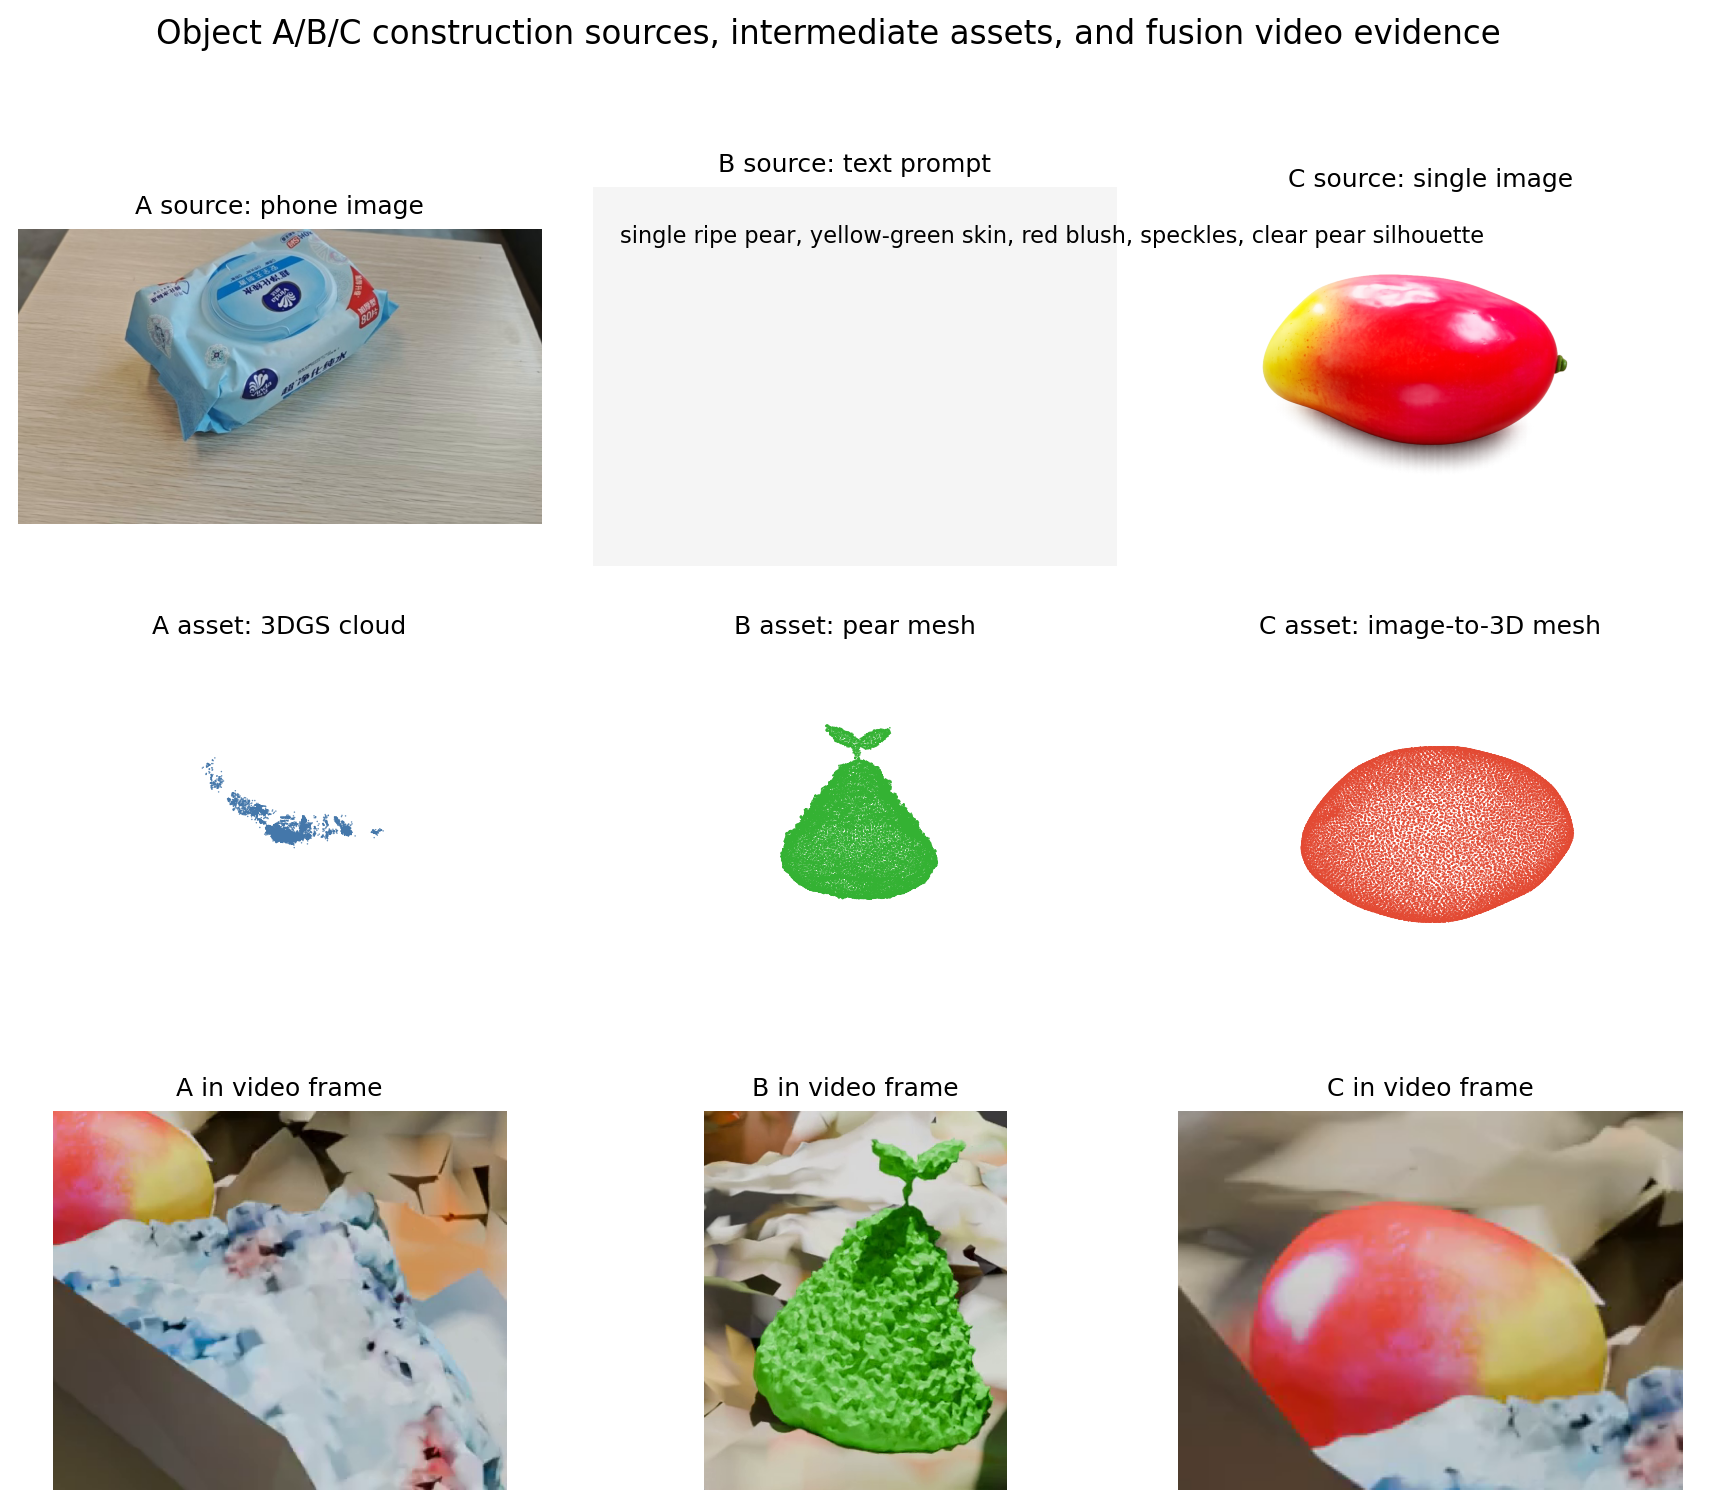
\includegraphics[width=0.96\textwidth]{task1_object_abc_construction.png}
    \caption{物体 A/B/C 的来源、三维资产与融合视频对应位置。A 为真实湿巾包重建，B 为梨形 text-to-3D 网格，C 为单图生成网格。}
    \label{fig:task1-object-abc-construction}
\end{figure}

真实物体 A 的 3DGS 训练日志保留了逐 step 的损失标量。图~\ref{fig:task1-object-a-loss} 展示了 \code{total\_loss} 与 \code{l1\_loss} 的变化：\code{total\_loss} 从第 1 step 的 0.1894 降至第 7000 step 的 0.0186，\code{l1\_loss} 从 0.1790 降至 0.0136。约 3000 和 6000 step 附近的短时尖峰后，曲线能迅速回到下降轨迹，说明自采物体 A 的 COLMAP+3DGS 训练已经形成稳定收敛趋势。

\begin{figure}[H]
    \centering
    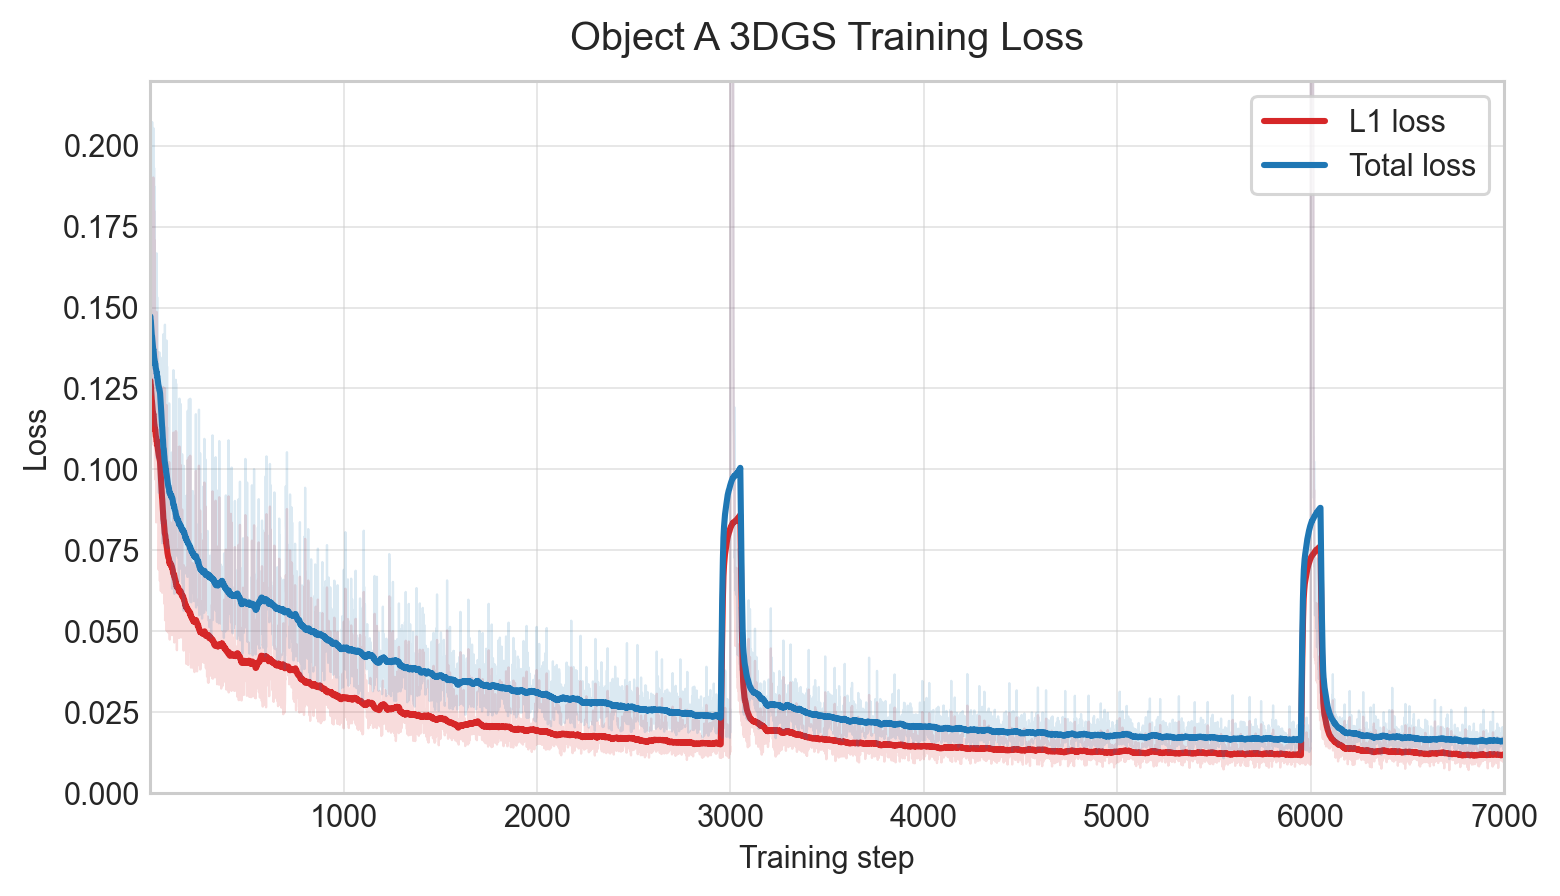
\includegraphics[width=0.78\textwidth]{task1_object_a_loss_curve.png}
    \caption{真实物体 A 的 3DGS 训练 loss 曲线}
    \label{fig:task1-object-a-loss}
\end{figure}

图~\ref{fig:task1-object-a-reconstruction} 进一步展示了真实物体 A 的采集和重建细节。左侧为手机多视角图像样例，可以看到物体主体在不同方位下均被覆盖；中间为 COLMAP 稀疏点云，主要恢复出物体外轮廓和局部纹理结构；右侧为 3DGS 训练后的高斯中心分布，相比稀疏点云更密集，能够作为后续几何资产整理和 Blender 融合的输入。该实验从自采图像出发完成 COLMAP、undistortion、3DGS 训练和点云导出，形成了完整的真实物体 A pipeline。

\begin{figure}[H]
    \centering
    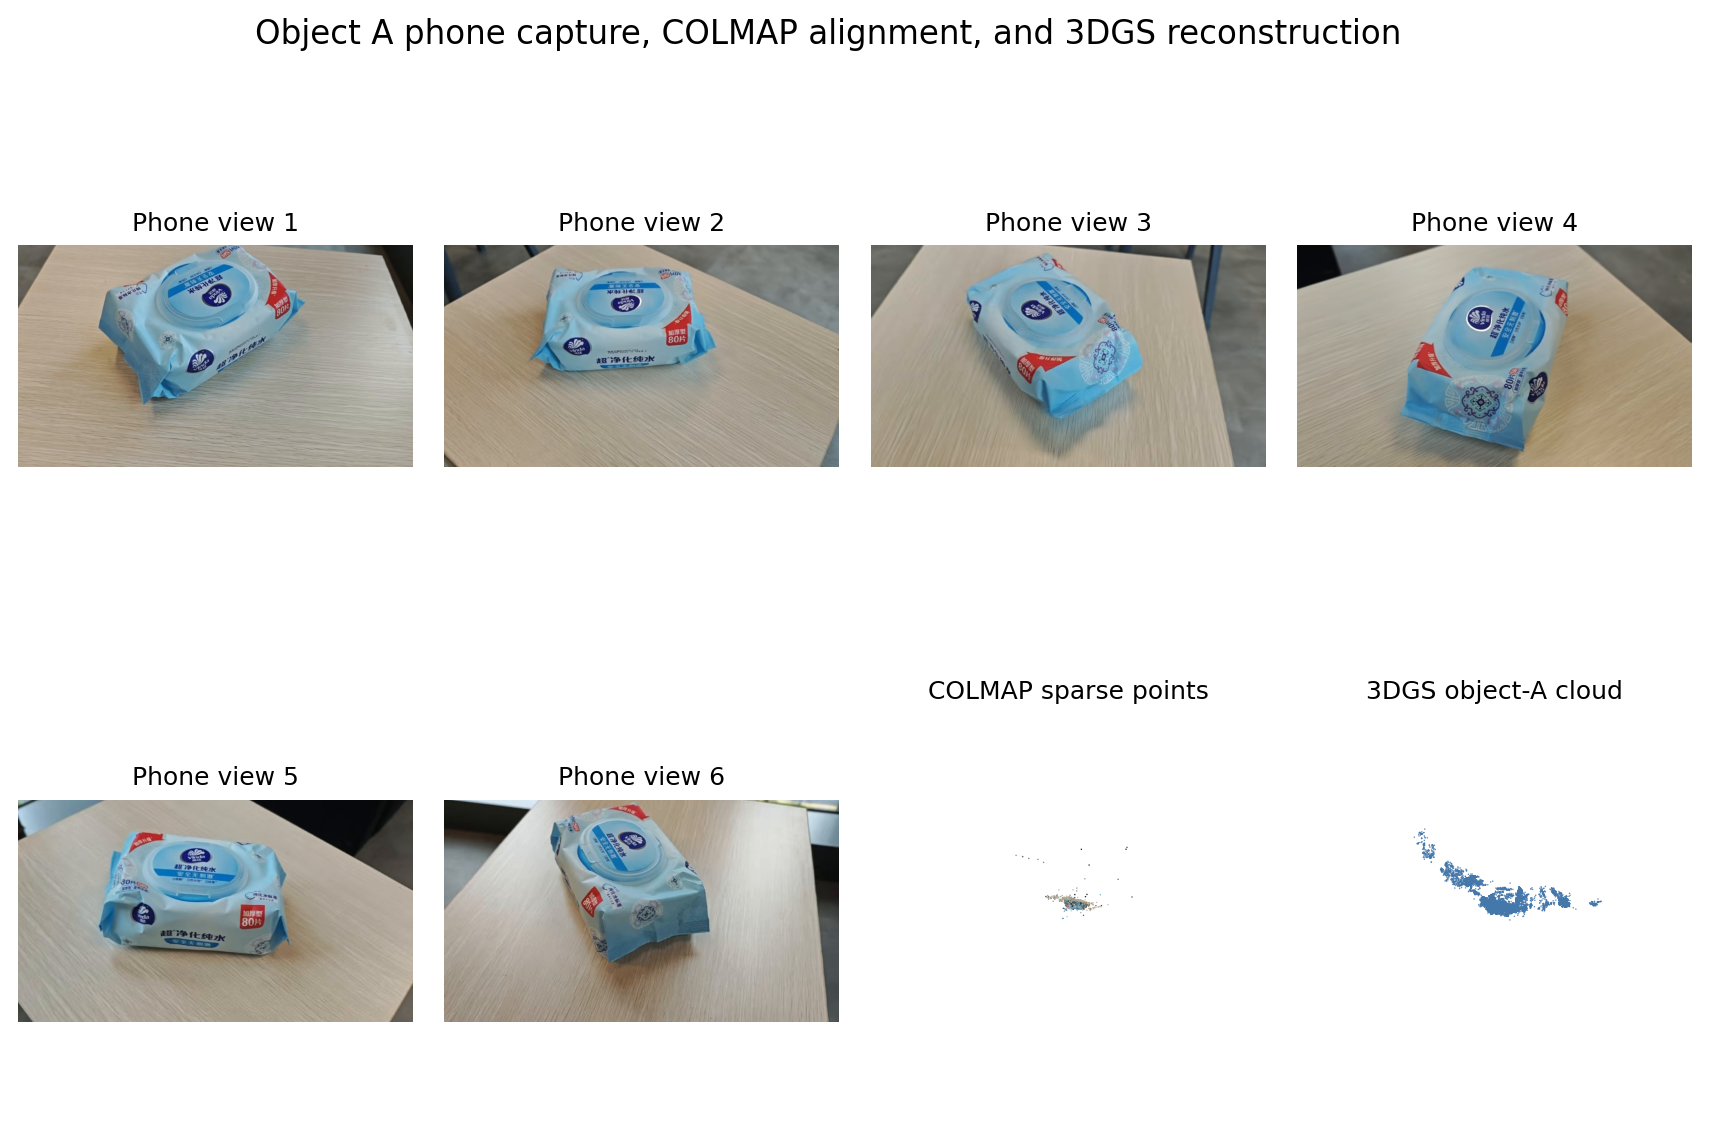
\includegraphics[width=0.96\textwidth]{task1_object_a_reconstruction.png}
    \caption{真实物体 A 的手机采集、COLMAP 稀疏重建与 3DGS 点云结果}
    \label{fig:task1-object-a-reconstruction}
\end{figure}

\subsection{Mip-NeRF 360 任务场景重建}
\label{subsec:task1-scenes}

场景重建部分使用 Mip-NeRF 360 数据集中的 \code{garden}、\code{bicycle} 和 \code{counter}。每个场景都包含原始图像、下采样图像和 COLMAP 稀疏重建结果。本文采用数据集附带的 COLMAP 相机与稀疏点云文件，使用官方 3DGS 训练代码读取这些文件完成训练，并在测试视角上计算 PSNR、SSIM 和 LPIPS。该部分对应题目一中的“任务场景重建”要求。

\begin{table}[!htbp]
    \centering
    \caption{Mip-NeRF 360 场景与 COLMAP 文件检查}
    \label{tab:scene-colmap-check}
    \small
    \begin{tabular}{lrrl}
        \toprule
        场景 & 原始图像数 & 下采样图像数 & COLMAP sparse/0 文件 \\
        \midrule
        garden & 185 & 185 & cameras.bin, images.bin, points3D.bin, points3D.ply \\
        bicycle & 194 & 194 & cameras.bin, images.bin, points3D.bin, points3D.ply \\
        counter & 240 & 240 & cameras.bin, images.bin, points3D.bin, points3D.ply \\
        \bottomrule
    \end{tabular}
\end{table}

3D Gaussian Splatting 将场景表示为一组可学习的三维高斯。每个高斯包含中心位置、尺度、旋转、不透明度和颜色相关参数。渲染时，模型将这些三维高斯投影到目标相机平面，并通过 alpha blending 合成图像。官方 3DGS 训练中使用图像重建损失优化场景参数，整体损失为
\begin{equation}
    \mathcal{L} = (1-\lambda)\mathcal{L}_{1} + \lambda \mathcal{L}_{D\text{-}SSIM},
\end{equation}
其中 \(\mathcal{L}_{1}\) 约束像素级重建误差，\(\mathcal{L}_{D\text{-}SSIM}\) 约束结构相似性。主实验对三个场景均训练 30000 iterations，图像分辨率下采样倍率为 4。

\begin{table}[!htbp]
    \centering
    \caption{3DGS 实验配置}
    \label{tab:3dgs-config}
    \small
    \begin{tabular}{ll}
        \toprule
        项目 & 设置 \\
        \midrule
        代码库 & Official 3D Gaussian Splatting \\
        数据集 & Mip-NeRF 360 garden, bicycle, counter \\
        输入几何 & COLMAP sparse camera/point files \\
        训练设备 & NVIDIA GeForce RTX 4090 D, 24GB \\
        主实验 iterations & 30000 \\
        主实验下采样倍率 & 4 \\
        评价指标 & PSNR, SSIM, LPIPS \\
        \bottomrule
    \end{tabular}
\end{table}

表~\ref{tab:3dgs-metrics} 给出了三个场景的主结果。\code{counter} 场景在三项指标中表现最好，PSNR 达到 29.61，SSIM 达到 0.9290，LPIPS 降到 0.1007；\code{garden} 场景也取得稳定重建效果；\code{bicycle} 场景指标相对较低，说明细长结构、遮挡和复杂纹理会增加 3DGS 新视角重建难度。

\begin{table}[!htbp]
    \centering
    \caption{3DGS 定量评价结果}
    \label{tab:3dgs-metrics}
    \small
    \begin{tabular}{llrrr}
        \toprule
        配置 & 场景 & PSNR $\uparrow$ & SSIM $\uparrow$ & LPIPS $\downarrow$ \\
        \midrule
        30000 steps, 下采样倍率 4 & bicycle & 25.6565 & 0.7794 & 0.2024 \\
        30000 steps, 下采样倍率 4 & counter & 29.6144 & 0.9290 & 0.1007 \\
        30000 steps, 下采样倍率 4 & garden & 27.8553 & 0.8751 & 0.1027 \\
        \bottomrule
    \end{tabular}
\end{table}

图~\ref{fig:garden-main}、图~\ref{fig:counter-main} 和图~\ref{fig:bicycle-main} 分别展示三个主场景的测试视角渲染结果。每张 contact sheet 中交替展示真实图像和渲染图像，便于观察局部结构、颜色和视角一致性。\code{counter} 的桌面、柜体和室内背景结构较稳定，与最高 SSIM 和较低 LPIPS 相符；\code{garden} 的地面和植被整体恢复较好，但局部植被细节会出现模糊；\code{bicycle} 中车轮、辐条和背景细纹理更容易产生不稳定渲染。

\begin{figure}[H]
    \centering
    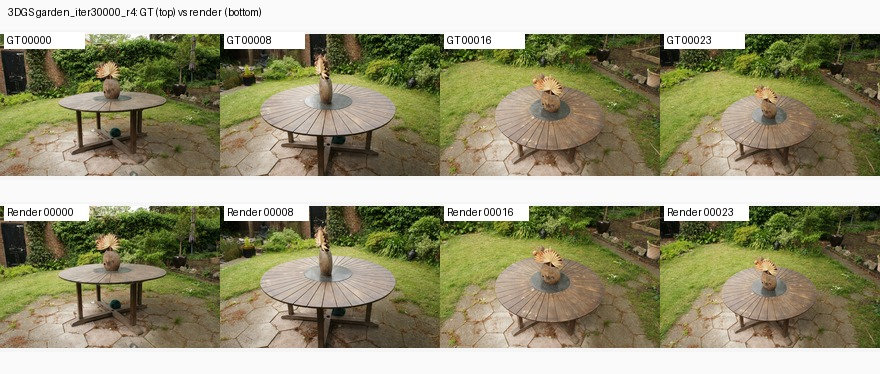
\includegraphics[width=\textwidth]{3dgs_garden_iter30000_r4_contact.jpg}
    \caption{\code{garden} 主实验测试视角渲染结果}
    \label{fig:garden-main}
\end{figure}

\begin{figure}[H]
    \centering
    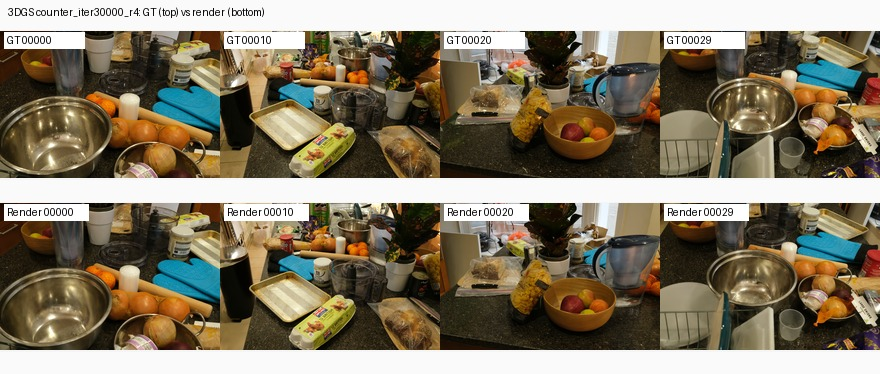
\includegraphics[width=\textwidth]{3dgs_counter_iter30000_r4_contact.jpg}
    \caption{\code{counter} 主实验测试视角渲染结果}
    \label{fig:counter-main}
\end{figure}

\begin{figure}[!htbp]
    \centering
    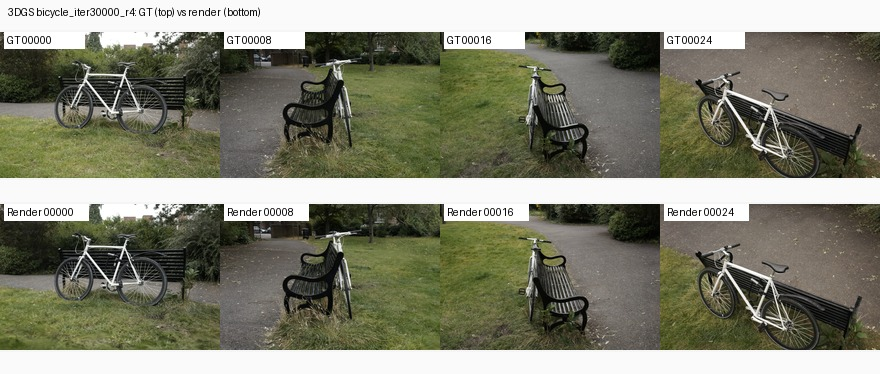
\includegraphics[width=\textwidth]{3dgs_bicycle_iter30000_r4_contact.jpg}
    \caption{\code{bicycle} 主实验测试视角渲染结果}
    \label{fig:bicycle-main}
\end{figure}

\subsection{A/B/C 与重建场景融合}
\label{subsec:task1-fusion}

场景融合阶段使用 \code{counter} 场景的 3DGS 采样点云进行 Poisson surface reconstruction，得到可导入 Blender 的背景 mesh。随后将物体 A 的湿巾模型、物体 B 的绿色梨形纹理网格和物体 C 的单图生成网格导入 Blender，并统一设置位姿、缩放、顶点颜色和贴图材质。最终渲染脚本使用固定中心环绕和先近后远的相机轨迹，导出 150 帧、24 fps、1280\(\times\)720 的 H.264 MP4 视频。

\subsubsection{3DGS 点云与 AIGC Mesh 的处理}

融合阶段首先需要分别处理两类三维资产。3DGS 重建资产的原始表达是高斯基元，适合新视角渲染，但不适合直接和传统 OBJ 网格在 Blender 中共同计算遮挡、材质和相机漫游。因此本文先从 3DGS 最终模型导出高斯中心或采样点云，保留空间坐标和颜色信息；随后使用 Open3D 对点云估计 KNN 邻域法向，并通过 Poisson 曲面重建生成连续三角网格。Poisson 重建后再依据顶点密度去除低置信度边缘区域，并用连通域筛选减少孤立碎片，最后导出 PLY/OBJ 网格作为 Blender 背景或真实物体资产。

AIGC 生成资产的处理方式不同。物体 B 和物体 C 已经由 text-to-3D 或 image-to-3D 流程导出为多边形网格，因此不再进行 Poisson 曲面重建，而是保留其 OBJ 几何和纹理图像，在 Blender 中完成坐标、朝向、尺度和材质绑定。物体 B 使用生成的梨形网格和纹理贴图，物体 C 使用单图生成网格和对应纹理贴图；二者通过 Image Texture 节点接入 Principled BSDF，从而保持 AIGC 资产原本的纹理外观。

\begin{table}[!htbp]
    \centering
    \caption{异构三维资产到统一 mesh 表达的转换流程}
    \label{tab:task1-unified-representation}
    \small
    \begin{tabularx}{\textwidth}{lX}
        \toprule
        阶段 & 实际处理 \\ 
        \midrule
        3DGS 场景/物体 & 高斯中心或采样点云 \(\rightarrow\) 法向估计 \(\rightarrow\) Poisson 曲面重建 \(\rightarrow\) 密度裁剪与连通域筛选 \(\rightarrow\) 顶点颜色 mesh \\ 
        AIGC 物体 B/C & text-to-3D 或 image-to-3D 导出的 OBJ mesh \(\rightarrow\) 坐标和尺度对齐 \(\rightarrow\) 纹理贴图绑定 \(\rightarrow\) 纹理 mesh \\ 
        Blender 统一输入 & 背景、物体 A、物体 B、物体 C 均以 mesh 对象进入同一场景，差异只保留在材质来源上 \\ 
        \bottomrule
    \end{tabularx}
\end{table}

\subsubsection{统一表达形式与联合渲染}

完成上述转换后，所有资产都以 mesh 形式进入 Blender，但材质来源保留各自特点。对于场景 surface mesh，脚本将采样点云颜色通过最近邻映射写入 \code{mesh.vertex\_colors}；对于物体 A 的 3DGS PLY，整理过程读取低阶球谐颜色分量并按 \(0.5+C_0 f_{dc}\) 恢复基础颜色，其中 \(C_0=0.2820947918\)，再写入顶点颜色属性。Blender 渲染脚本对 \code{TABLE} 和 \code{tissue} 调用顶点颜色材质，对 \code{Obj\_B} 和 \code{Obj\_C} 绑定纹理图像；因此四类资产能够共享同一坐标系、同一相机轨迹和同一 Cycles 光照环境，并在视频中形成统一的遮挡关系。

\begin{table}[!htbp]
    \centering
    \caption{A/B/C 场景融合视频设置}
    \label{tab:task1-object-a-fusion}
    \small
    \begin{tabularx}{\textwidth}{lX}
        \toprule
        项目 & 设置与结果 \\
        \midrule
        背景场景 & 使用 \code{counter} 的 3DGS 采样点云重建 Poisson surface mesh \\
        物体 A & 真实湿巾包 COLMAP+3DGS 重建资产 \\
        物体 B & text-to-3D 梨形纹理网格 \\
        物体 C & Zero123 单图生成网格 \\
        坐标与材质 & A/B/C 与背景 mesh 在 Blender 中统一坐标摆放，并绑定顶点颜色或贴图材质 \\
        漫游视频 & 150 frames, 24 fps, 1280\(\times\)720, H.264 MP4 \\
        \bottomrule
    \end{tabularx}
\end{table}

图~\ref{fig:task1-blender-fusion} 抽取了视频中的六个关键帧，可以看到三个物体被放置在重建背景上，并且环绕视角能展示它们相对背景的空间位置。该结果对应题目一要求中的“将 A/B/C 放入重建背景场景并生成漫游视频”。

\begin{figure}[!htbp]
    \centering
    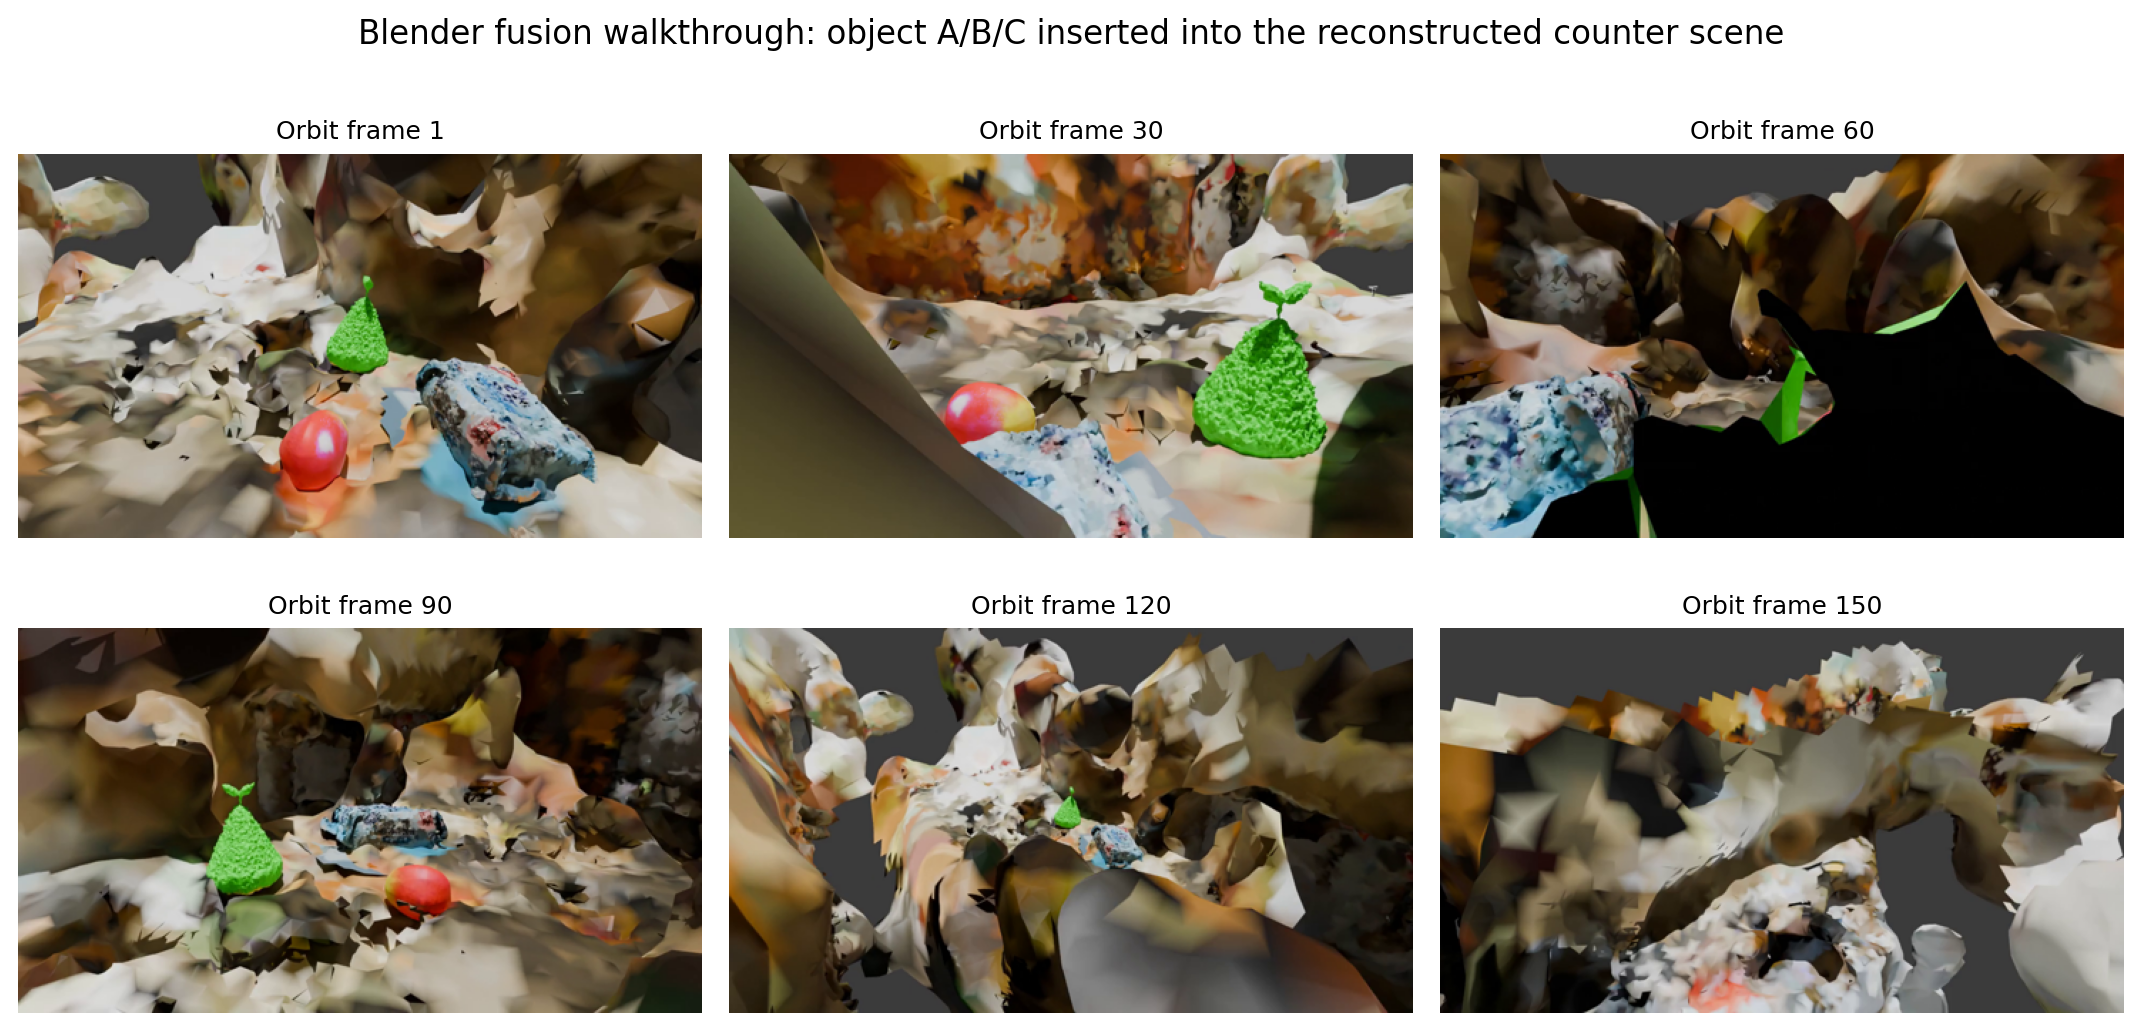
\includegraphics[width=0.96\textwidth]{task1_blender_fusion_video_frames.png}
    \caption{Blender 中将物体 A、梨形物体 B 和单图生成物体 C 插入重建 \code{counter} 背景后的漫游视频抽帧}
    \label{fig:task1-blender-fusion}
\end{figure}

\subsection{消融实验与结果讨论}
\label{subsec:task1-supplement}

除题目一主线要求外，本文还整理了训练步数、下采样倍率、点云/网格导出和 AIGC 路线示例，用于解释重建质量和生成路线。这些内容不打断前面三项任务，因此集中放在本节。

首先，\code{garden} 场景的训练步数消融显示，更长训练可以稳定改善图像质量。随着训练步数从 7000 增加到 30000，PSNR 从 26.62 提升到 27.86，SSIM 从 0.8395 提升到 0.8751，LPIPS 从 0.1528 降到 0.1027。下采样倍率 8 的指标更高，但这是在更低分辨率下得到的结果，说明低分辨率更容易拟合，并不代表高频细节一定优于下采样倍率 4。

\begin{table}[!htbp]
    \centering
    \caption{\code{garden} 场景训练步数与分辨率消融实验}
    \label{tab:garden-steps}
    \small
    \begin{tabular}{lrrr}
        \toprule
        配置 & PSNR $\uparrow$ & SSIM $\uparrow$ & LPIPS $\downarrow$ \\
        \midrule
        7000 steps, 下采样倍率 4 & 26.6160 & 0.8395 & 0.1528 \\
        15000 steps, 下采样倍率 4 & 27.3543 & 0.8657 & 0.1142 \\
        30000 steps, 下采样倍率 4 & 27.8553 & 0.8751 & 0.1027 \\
        30000 steps, 下采样倍率 8 & 29.7440 & 0.9252 & 0.0548 \\
        \bottomrule
    \end{tabular}
\end{table}

\begin{figure}[!htbp]
    \centering
    \begin{subfigure}{0.32\textwidth}
        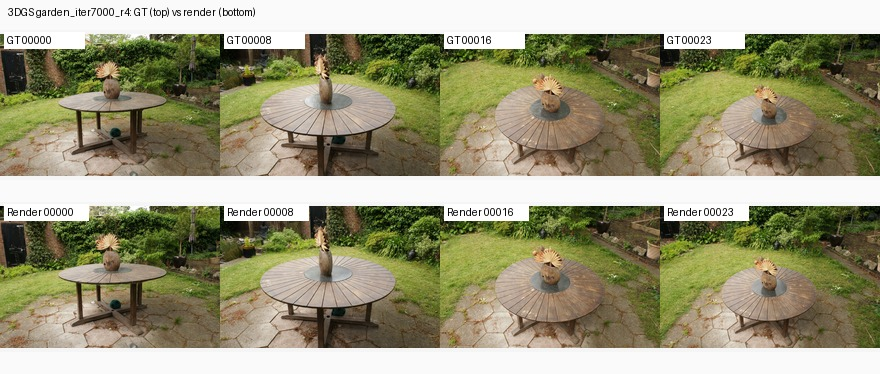
\includegraphics[width=\textwidth]{3dgs_garden_iter7000_r4_contact.jpg}
        \caption{7000 steps}
    \end{subfigure}
    \hfill
    \begin{subfigure}{0.32\textwidth}
        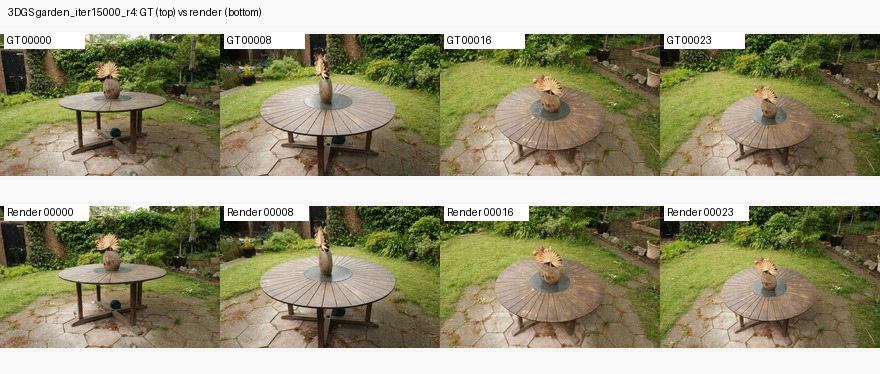
\includegraphics[width=\textwidth]{3dgs_garden_iter15000_r4_contact.jpg}
        \caption{15000 steps}
    \end{subfigure}
    \hfill
    \begin{subfigure}{0.32\textwidth}
        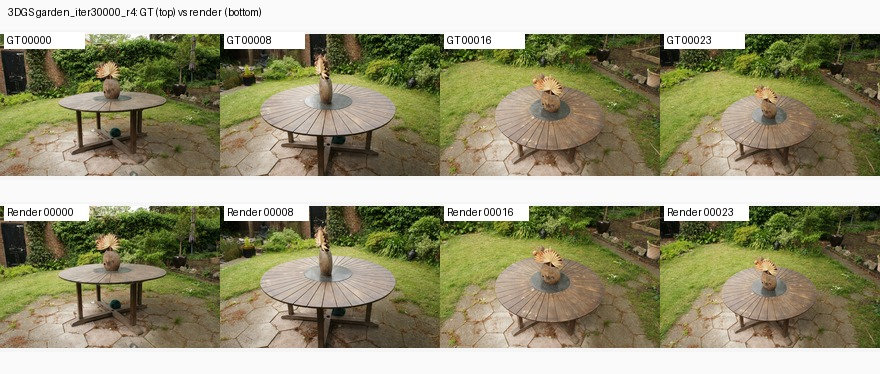
\includegraphics[width=\textwidth]{3dgs_garden_iter30000_r4_contact.jpg}
        \caption{30000 steps}
    \end{subfigure}
    \caption{\code{garden} 场景不同训练步数下的渲染对比}
    \label{fig:garden-step-ablation}
\end{figure}

\begin{figure}[!htbp]
    \centering
    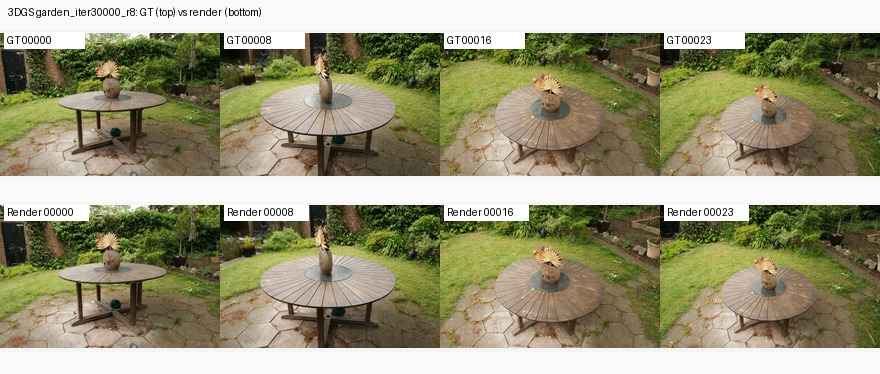
\includegraphics[width=0.96\textwidth]{3dgs_garden_iter30000_r8_contact.jpg}
    \caption{\code{garden} 下采样倍率 8 的低分辨率训练与渲染结果}
    \label{fig:garden-r8}
\end{figure}

其次，为了从三维资产角度检查 3DGS 输出，本文将三个主场景最终模型中的高斯中心采样为点云，并进一步用 Poisson surface reconstruction 生成表面网格。图~\ref{fig:blender-pointcloud} 和图~\ref{fig:surface-mesh} 展示了点云和网格结果。它们不替代新视角图像指标，但能进一步说明重建结果已经可以被整理成 Blender 中可观察的三维资产。

\begin{figure}[H]
    \centering
    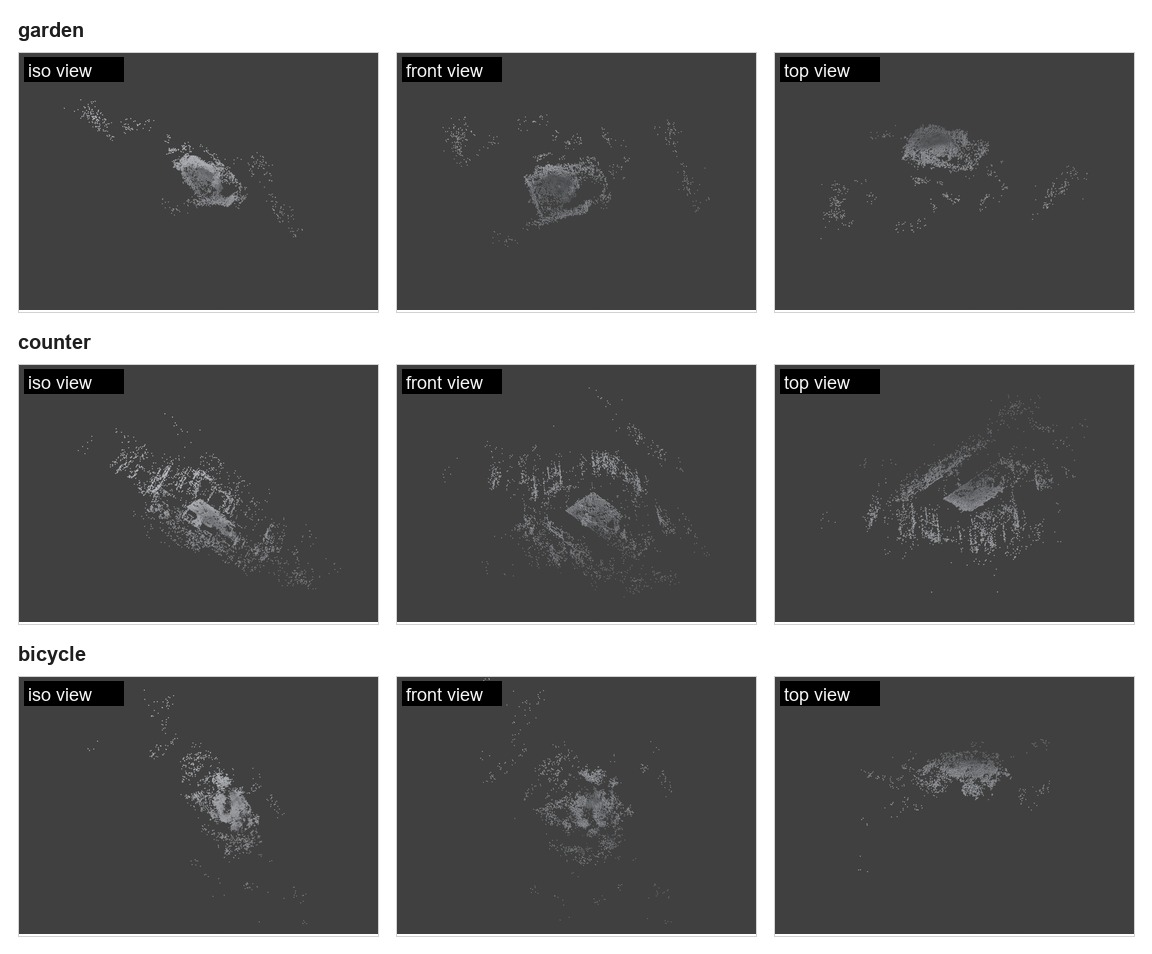
\includegraphics[width=0.90\textwidth]{3dgs_blender_pointcloud_contact.jpg}
    \caption{最终 3DGS 点云的 Blender 多视角展示}
    \label{fig:blender-pointcloud}
\end{figure}

\begin{figure}[H]
    \centering
    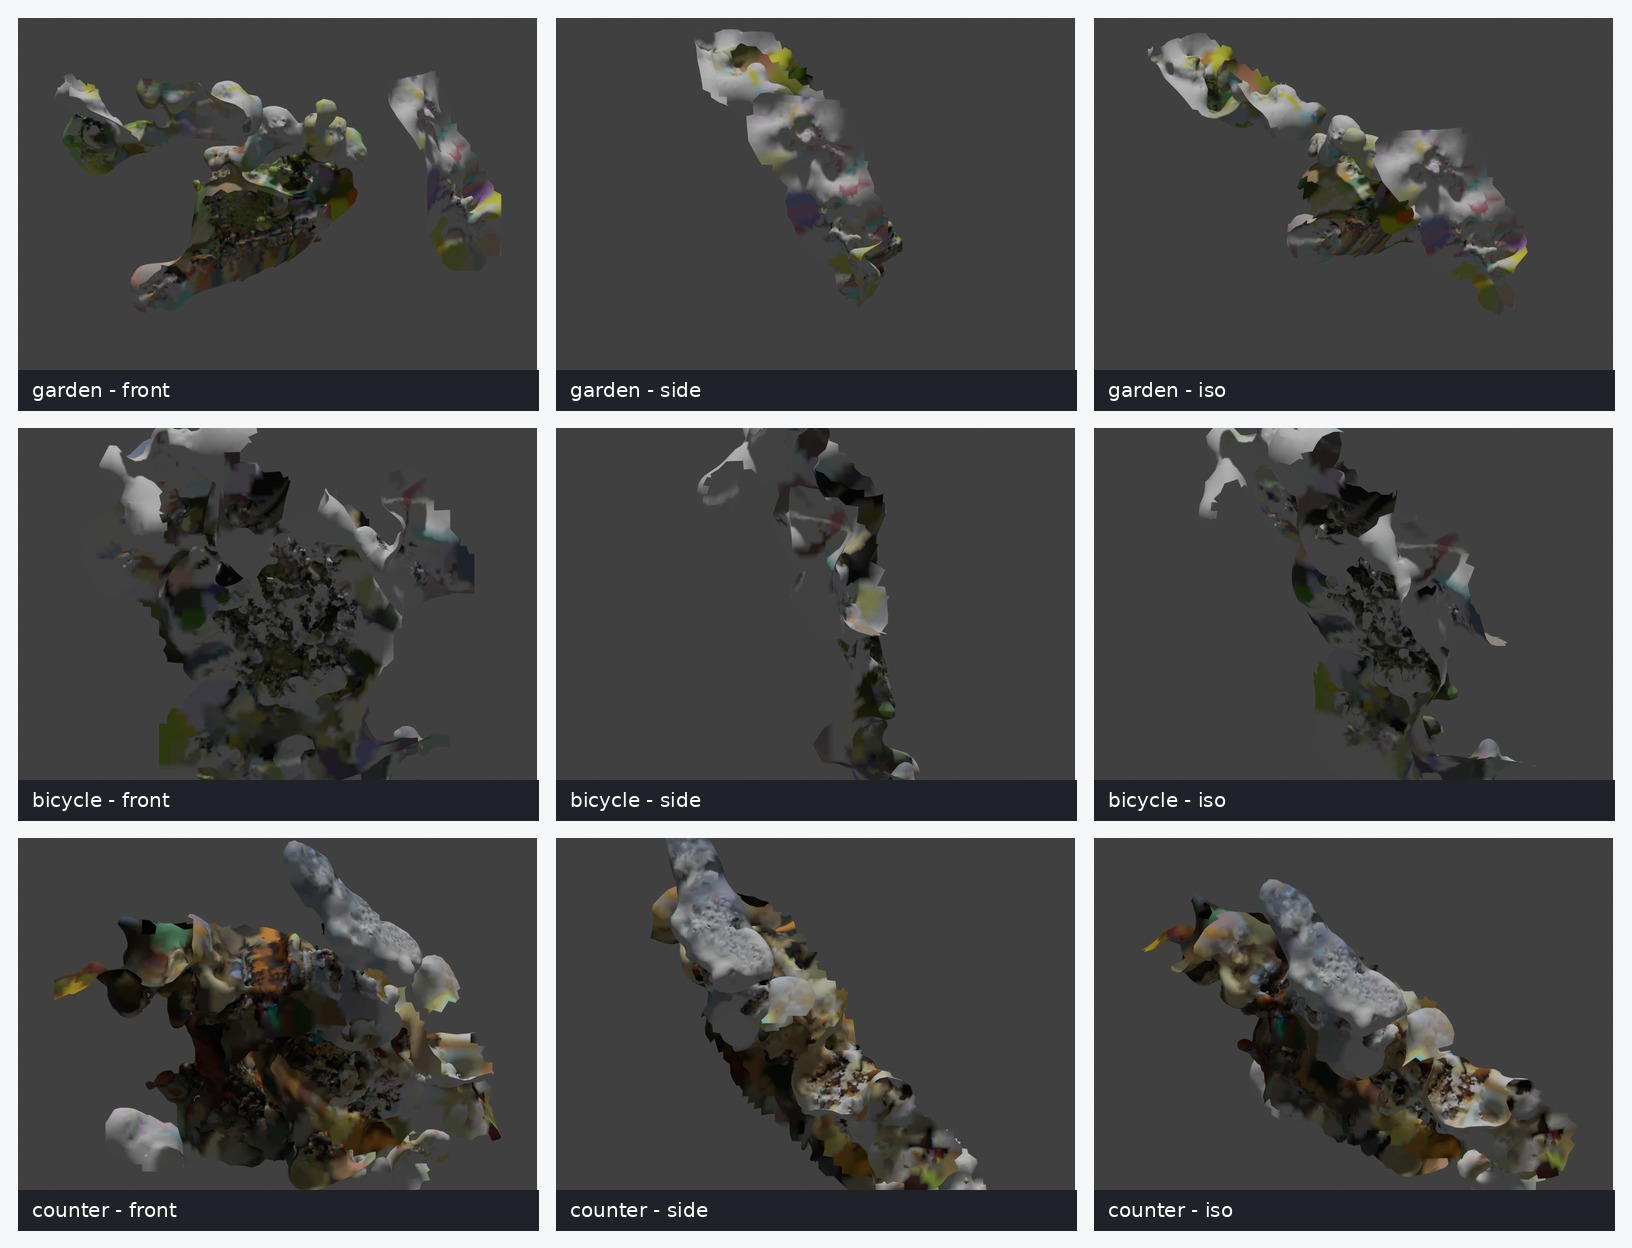
\includegraphics[width=0.86\textwidth]{3dgs_surface_mesh_contact.jpg}
    \caption{最终 3DGS 表面网格的 Blender 多视角展示}
    \label{fig:surface-mesh}
\end{figure}

最后，报告保留了一组 AIGC 生成路线示例，如图~\ref{fig:aigc-contact} 所示。该示例用于展示 threestudio SDS 与 Zero123 两条生成路线的可复现流程，帮助说明 text-to-3D 和 image-to-3D 的输出形式。

\begin{figure}[H]
    \centering
    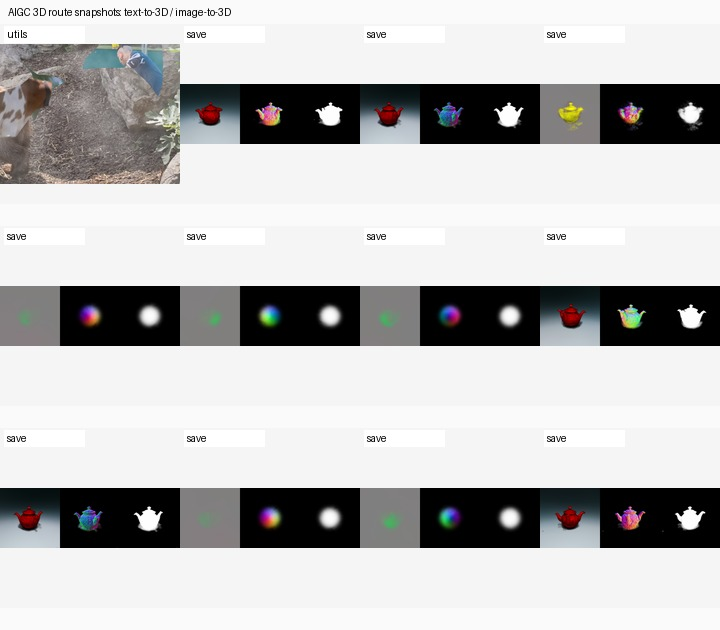
\includegraphics[width=0.62\textwidth]{aigc_output_contact.jpg}
    \caption{text-to-3D 与 image-to-3D 生成路线示例}
    \label{fig:aigc-contact}
\end{figure}

从结果看，真实多视角监督和生成式先验解决的是两个不同问题。3DGS 依赖多视角图像、相机位姿和稀疏几何输入，能够得到稳定、可度量的场景重建结果；AIGC 三维生成依赖文本或图像条件，适合在给定概念或单图条件下快速得到三维资产草图。最终融合部分把二者连接起来，重点体现从真实采集、生成资产、场景重建到 Blender 漫游视频的完整链路。

\section{LeRobot ACT 策略学习实验}

\subsection{基础策略训练}

题目二首先要求在 CALVIN 环境 A 上训练一个基础 ACT 策略。该策略只使用 \code{splitA} 数据，作用是建立单环境视觉--动作基线；后续 ABC-mixed 策略、chunk size 实验和条件输入实验都与它使用同一套评测协议，从而保证 zero-shot 对比有明确参照。

实验使用 LeRobot 格式的 CALVIN ABC-D 数据。为保证环境标签来源明确，本文先核验 \path{huiwon/calvin_task_ABC_D} 中的 \code{original\_frame\_idx} 与 CALVIN 官方 \code{task\_ABC\_D} 的 \code{scene\_info} 区间对应关系，并据此得到 scene-info 对齐的 A/B/C 标签。最终主分析采用 \path{xiaoma26/calvin-lerobot} 的显式划分数据：\code{splitA}、\code{splitB}、\code{splitC} 和 \code{splitD} 分别对应四个环境，其中 \code{splitA} 用于基础策略训练，\code{splitA/B/C} 合并后用于混合策略训练，\code{splitD} 只用于 zero-shot 评测。该数据中 \code{splitA} 含 6089 个 episode、366693 帧，\code{splitB} 含 6115 个 episode、367096 帧，\code{splitC} 含 5666 个 episode、337954 帧，\code{splitD} 含 5124 个 episode、308918 帧。

\begin{figure}[!htbp]
    \centering
    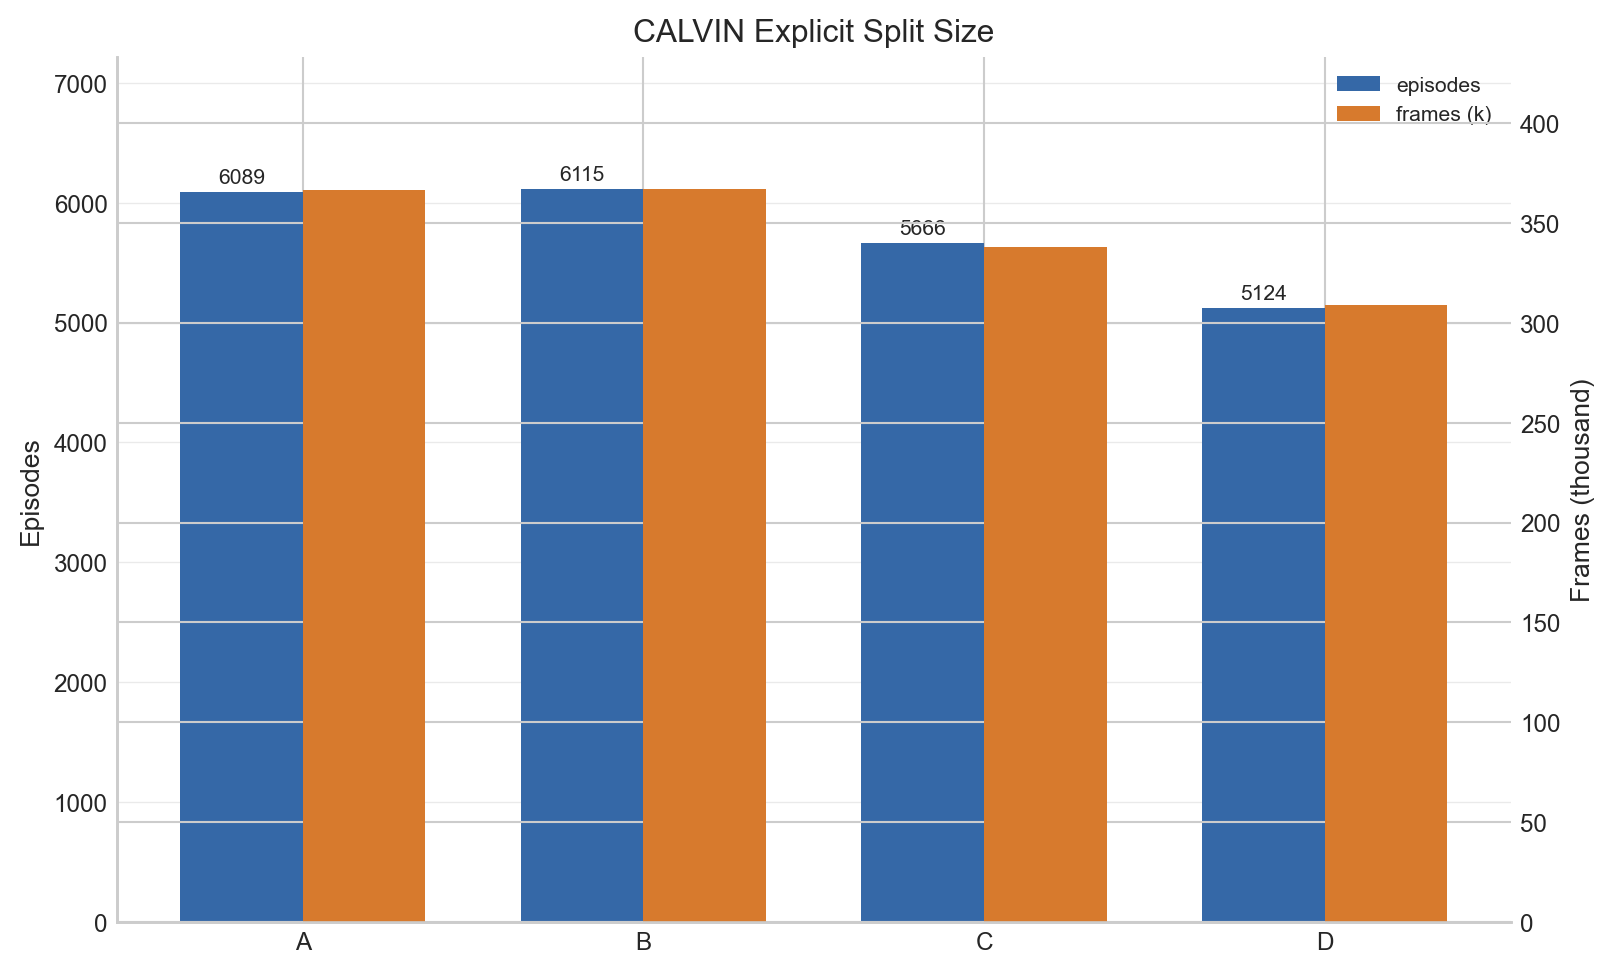
\includegraphics[width=0.82\textwidth]{task2_split_size.png}
    \caption{课程提供的 CALVIN splitA/B/C/D 数据规模}
    \label{fig:task2-split-size}
\end{figure}

图~\ref{fig:task2-split-size} 展示了主分析所用 split 的数据规模。A/B/C 三个训练环境的 episode 数和帧数接近，D 测试环境略小；因此基础策略和混合策略的差异主要来自训练环境覆盖范围、任务条件表示和训练过程，而不是某个 split 的数量级差异。

\begin{figure}[!htbp]
    \centering
    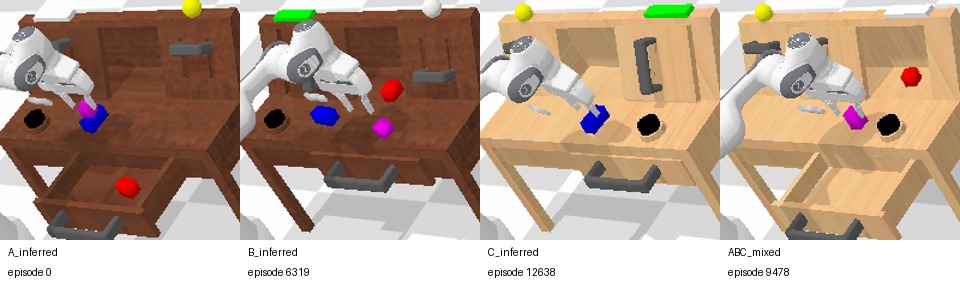
\includegraphics[width=0.92\textwidth]{task2_ordered_abc_split_samples.jpg}
    \caption{CALVIN ABC 训练集有序划分的图像抽样检查}
    \label{fig:task2-split-samples}
\end{figure}

\subsection{混合策略训练}

混合策略训练对应题目二的第二个核心要求：将 \code{splitA}、\code{splitB} 和 \code{splitC} 合并为 ABC-mixed 数据集，并在相同 ACT 框架下训练多环境策略。合并时，本文将三个 split 中的任务编号映射到同一套任务语义索引，避免相同任务在不同环境中编号不一致。模型输入包括 static camera、wrist camera、机器人状态和 task condition，输出为 7 维连续动作。

表~\ref{tab:act-config} 给出了基础策略和混合策略共用的主要训练设置。ACT（Action Chunking Transformer）不是逐步预测单个动作，而是在每个观测下预测一段未来动作序列；主实验采用 chunk size 50。为公平比较 A-only 与 ABC-mixed，二者使用相同网络结构、batch size、学习率、优化器、动作维度和在线评测环境。除主对比外，本文还加入更长训练、不同 chunk size、语言条件和错误条件输入等实验，用于分析性能差异来自数据混合、条件表示还是 checkpoint 选择。

\begin{table}[!htbp]
    \centering
    \caption{LeRobot ACT 主要训练设置}
    \label{tab:act-config}
    \small
    \begin{tabular}{ll}
        \toprule
        项目 & 设置 \\
        \midrule
        数据集 & CALVIN ABC-D LeRobot 格式数据 \\
        策略模型 & ACT \\
        Network architecture & CNN visual encoders + Transformer policy + action chunk decoder \\
        观测 & Static camera, wrist camera, robot state, task one-hot \\
        动作维度 & 7 \\
        Batch size & 8 \\
        Optimizer & AdamW \\
        Learning rate & 0.0001 \\
        Epochs / steps & step-based training, 主实验 50000/100000 steps \\
        扩展训练步数 & 120000--200000 checkpoint sweep, seed1 robustness check \\
        Loss function & Action L1 loss for continuous 7D action prediction \\
        主实验 chunk size & 50 \\
        评价环境 & CALVIN D zero-shot online evaluation \\
        \bottomrule
    \end{tabular}
\end{table}

\begin{figure}[!htbp]
    \centering
    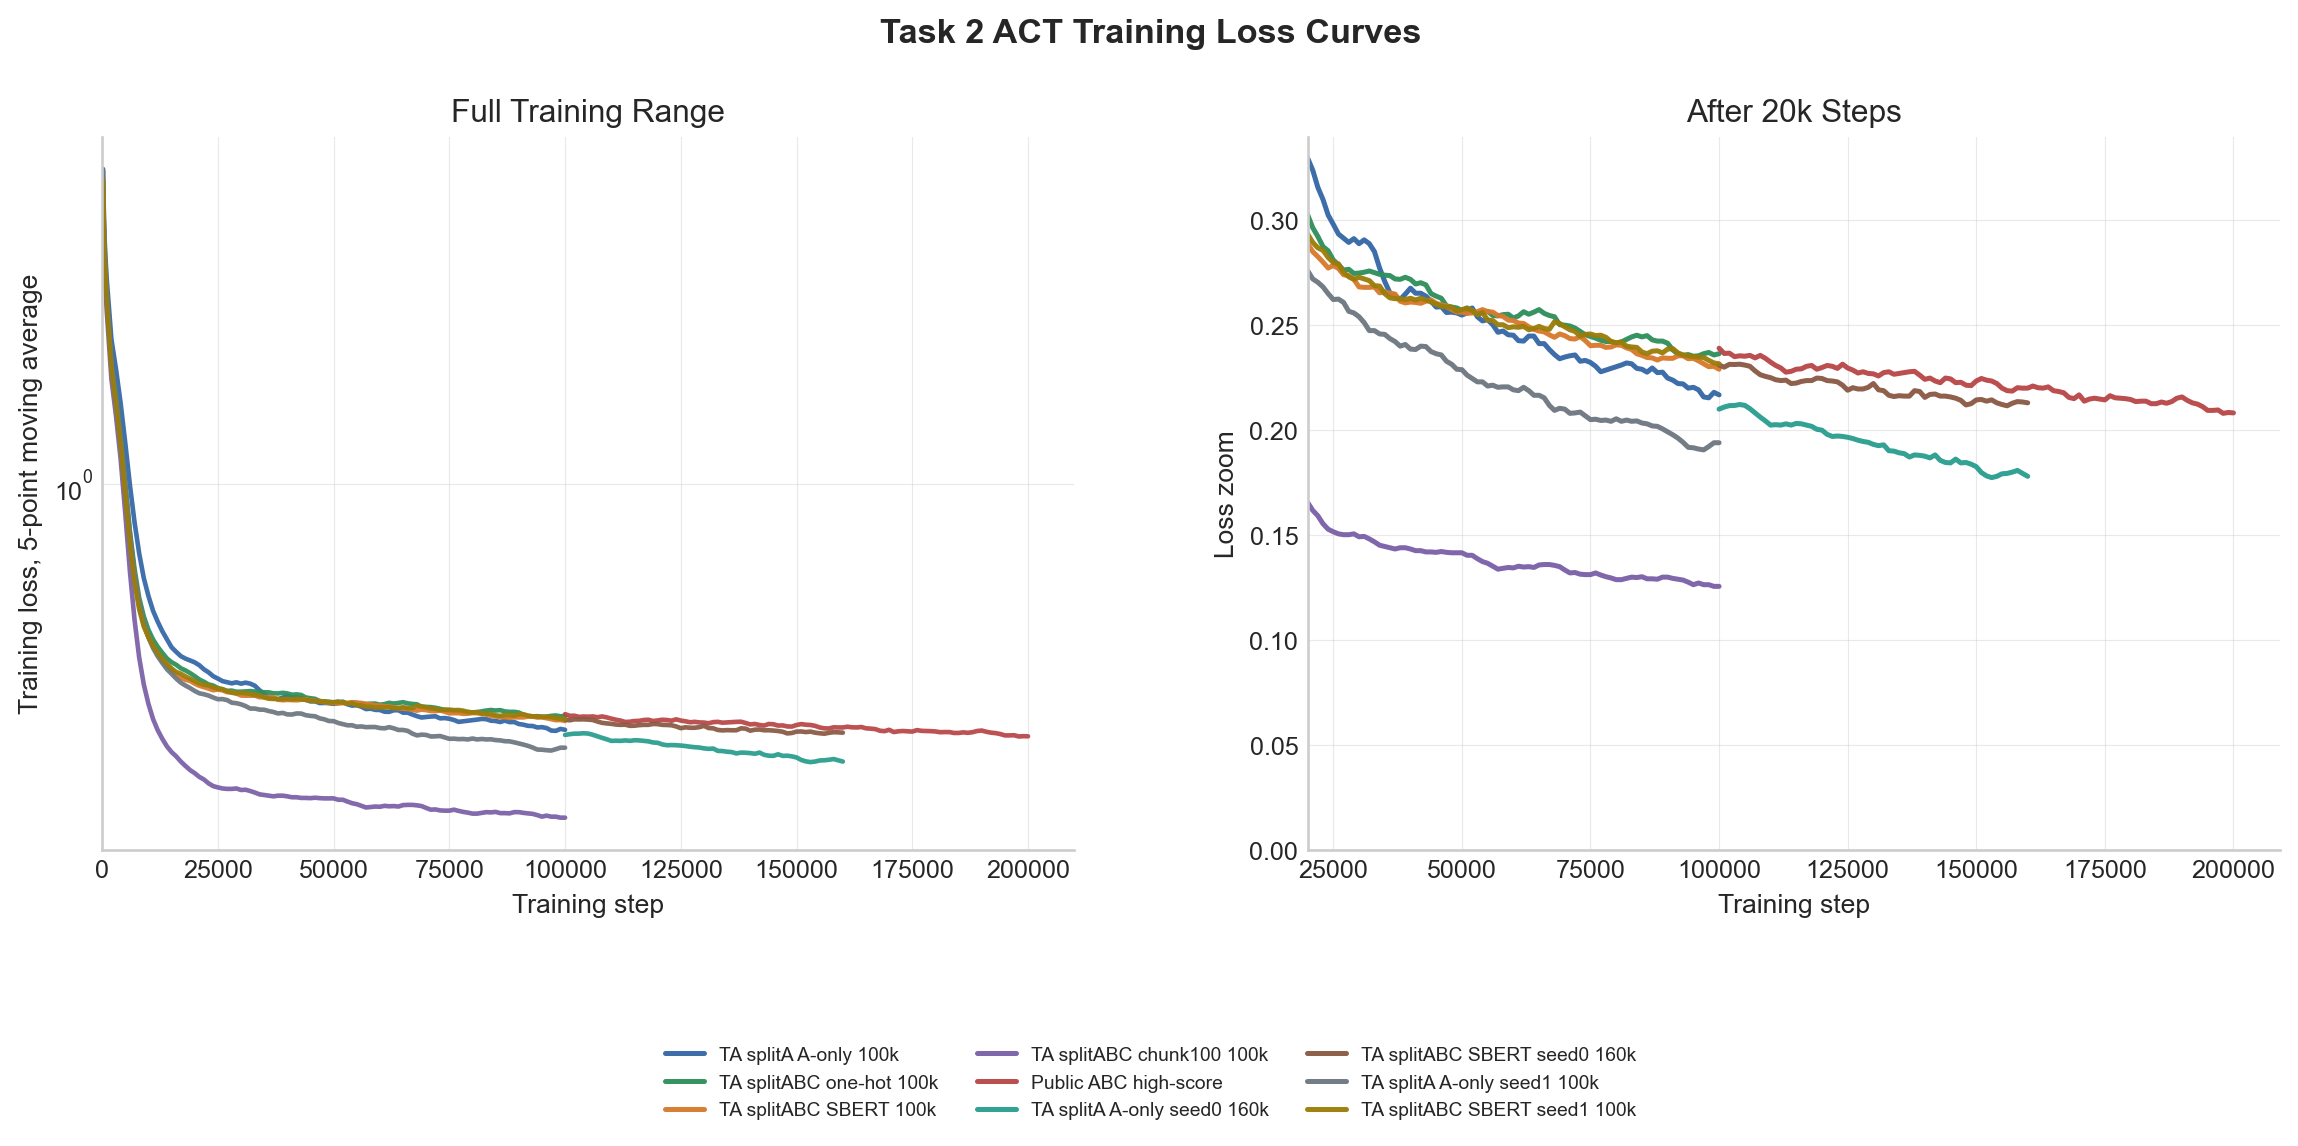
\includegraphics[width=0.92\textwidth]{task2_loss_curves.png}
    \caption{不同 ACT 实验训练过程中的 loss 曲线}
    \label{fig:task2-loss}
\end{figure}

图~\ref{fig:task2-loss} 根据训练日志中的 step-loss 记录绘制；训练时采用 \code{WANDB\_MODE=offline} 保存离线记录，并从本地日志导出报告曲线。图中使用 5 点滑动平均减少短期抖动，包含显式 split 主实验、ABC 扩展训练、A-only/SBERT 的 160000 step sweep，以及 seed1 稳健性训练。各模型的训练 loss 在前期快速下降，随后进入较平缓阶段。由于训练 loss 只反映示范动作拟合程度，后续仍需结合 CALVIN D 在线评测、任务条件表示和 checkpoint 选择判断真实泛化能力。

\subsection{Zero-shot 测试与成功率对比}

Zero-shot 测试阶段不再使用环境 D 的训练数据，而是把 A-only 和 ABC-mixed 策略直接部署到 CALVIN D。在线评测以连续完成子任务的长度作为主要指标。Avg Len 表示平均成功子任务数，SR@1 到 SR@5 分别表示至少完成 1 到 5 个连续子任务的比例。表~\ref{tab:act-main-results} 给出了与题目要求最直接对应的 A-only 与 ABC-mixed 对比。

\begin{table}[!htbp]
    \centering
    \caption{A-only 与 ABC-mixed ACT 在 CALVIN D 上的 zero-shot 对比}
    \label{tab:act-main-results}
    \small
    \begin{tabularx}{\textwidth}{Xrrrrrrr}
        \toprule
        模型 & Steps & Chunk & Avg Len & SR@1 & SR@2 & SR@3 & SR@5 \\
        \midrule
        \code{huiwon} A-only & 50000 & 50 & 0.288 & 0.229 & 0.048 & 0.011 & 0.000 \\
        \code{huiwon} ABC-mixed & 50000 & 50 & 0.278 & 0.236 & 0.037 & 0.005 & 0.000 \\
        \code{huiwon} A-only & 100000 & 50 & 0.407 & 0.316 & 0.078 & 0.013 & 0.000 \\
        \code{huiwon} ABC-mixed & 100000 & 50 & 0.303 & 0.242 & 0.056 & 0.005 & 0.000 \\
        \code{splitA} A-only & 100000 & 50 & 0.855 & 0.525 & 0.225 & 0.072 & 0.008 \\
        \code{splitABC} one-hot & 100000 & 50 & 0.649 & 0.402 & 0.165 & 0.052 & 0.009 \\
        \code{splitABC} SBERT & 100000 & 50 & 0.787 & 0.477 & 0.195 & 0.071 & 0.012 \\
        \code{splitA} A-only seed1 & 100000 & 50 & 0.846 & 0.487 & 0.219 & 0.088 & 0.011 \\
        \code{splitABC} SBERT seed1 & 100000 & 50 & 0.923 & 0.496 & 0.235 & 0.112 & 0.021 \\
        \code{splitA} A-only sweep & 160000 & 50 & 0.774 & 0.482 & 0.185 & 0.069 & 0.009 \\
        \code{splitABC} SBERT sweep & 160000 & 50 & 0.915 & 0.483 & 0.261 & 0.104 & 0.022 \\
        ABC extended 120k & 120000 & 50 & 1.028 & 0.561 & 0.277 & 0.119 & 0.022 \\
        \bottomrule
    \end{tabularx}
\end{table}

\begin{figure}[!htbp]
    \centering
    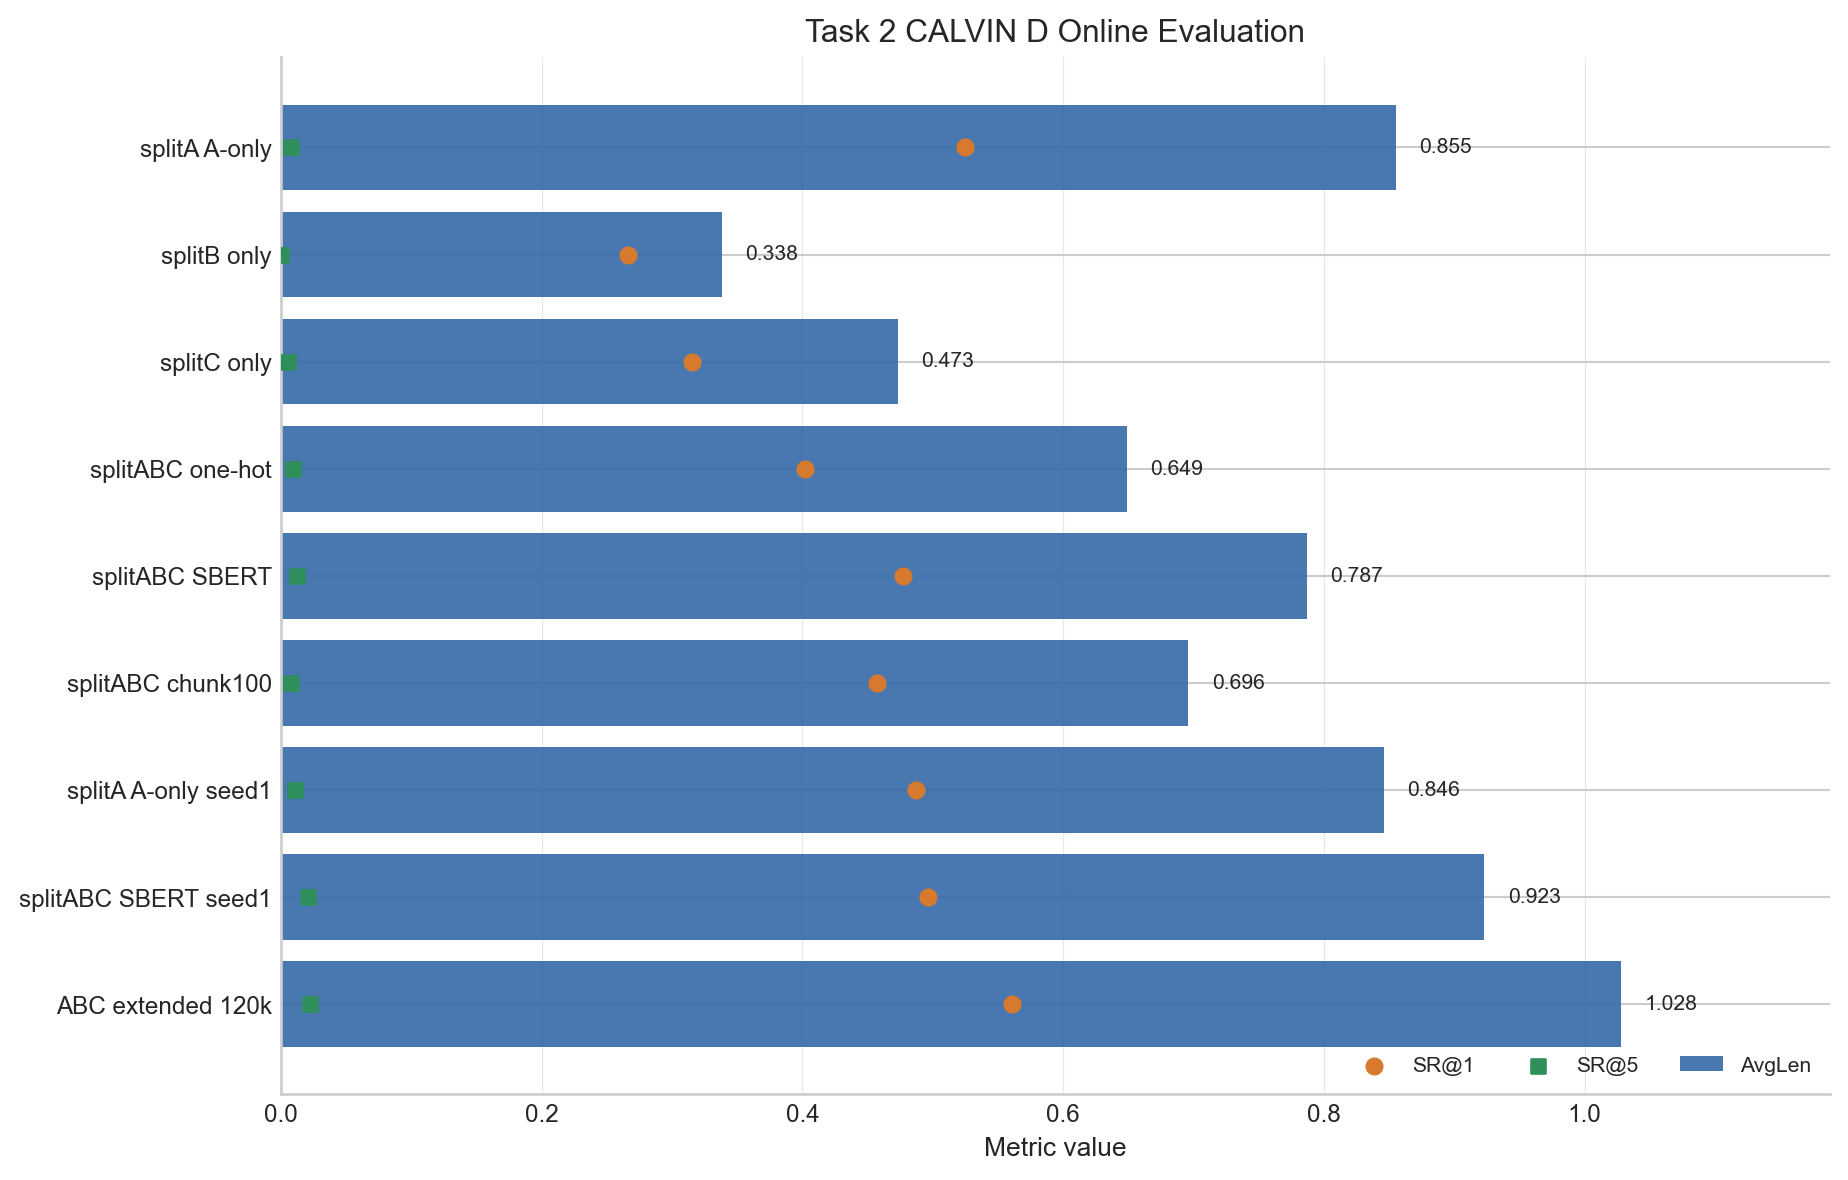
\includegraphics[width=0.96\textwidth]{task2_main_results_bar.png}
    \caption{主要 ACT 策略在 CALVIN D 上的 Avg Len 与成功率对比}
    \label{fig:task2-main-results-bar}
\end{figure}

\begin{figure}[!htbp]
    \centering
    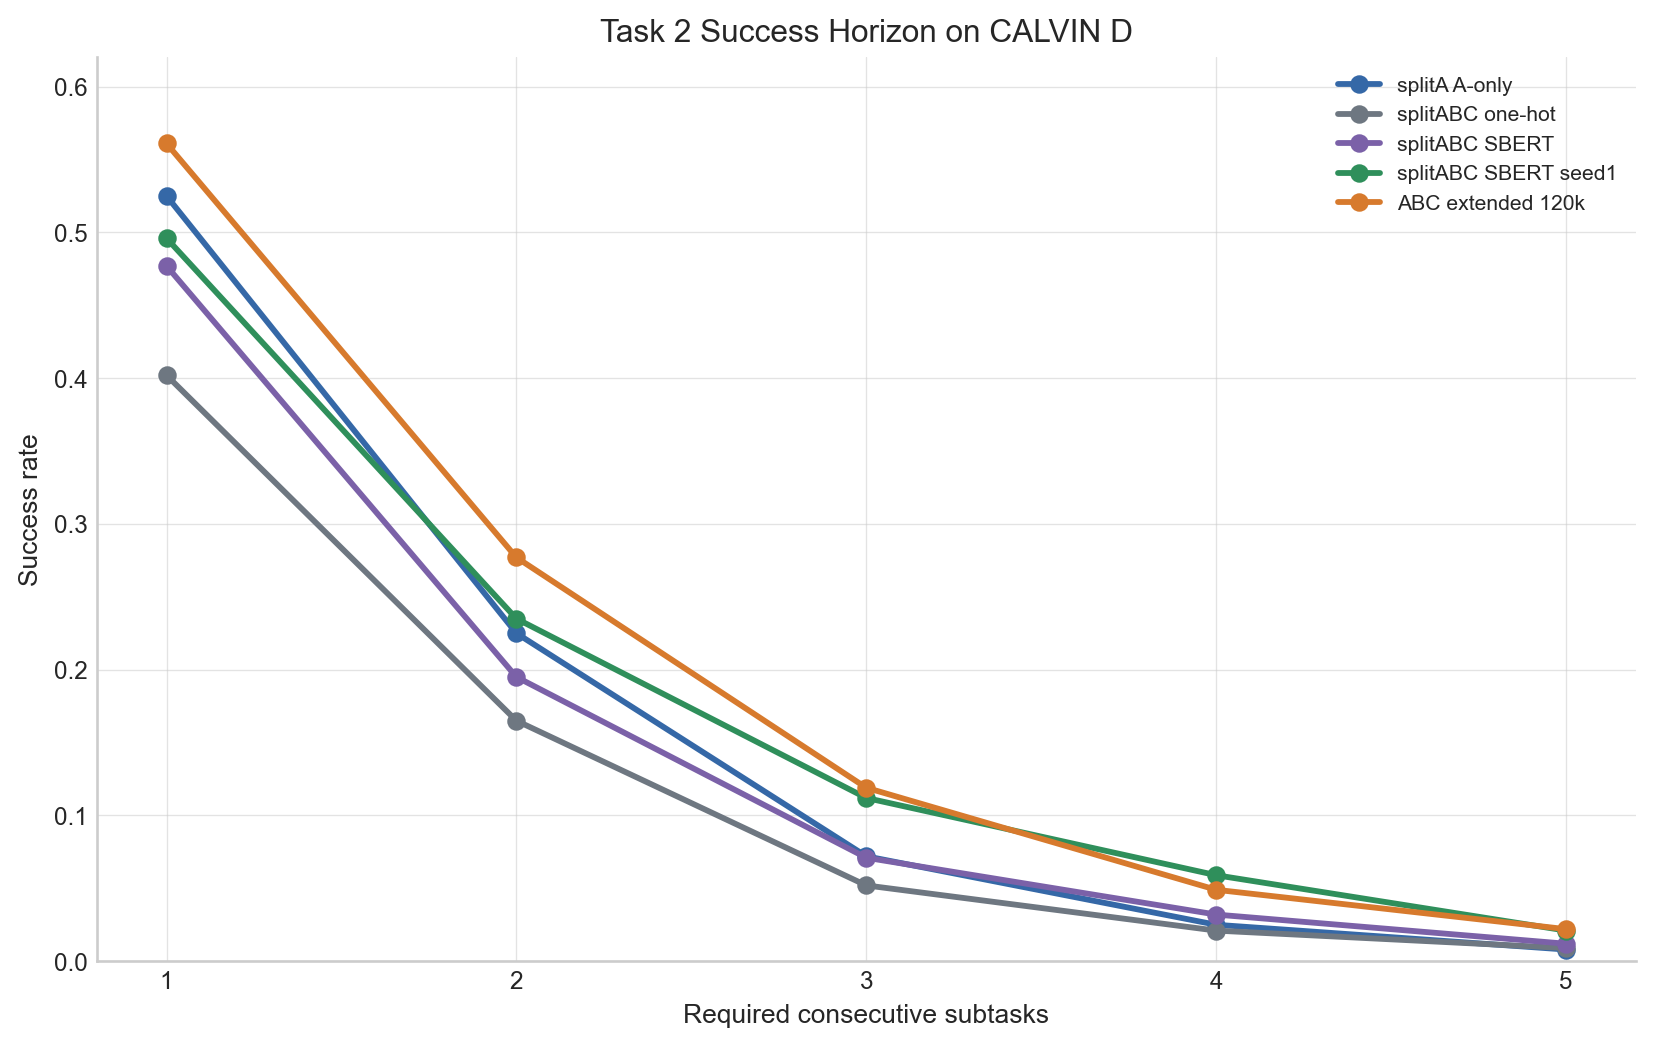
\includegraphics[width=0.96\textwidth]{task2_success_horizon.png}
    \caption{不同策略的连续成功深度曲线}
    \label{fig:task2-success-horizon}
\end{figure}

在 scene-info 对齐数据上，A-only 与 ABC-mixed 使用相同 ACT 结构、训练预算和 chunk size 50。50000 step 主实验中，A-only 的 Avg Len 为 0.288，ABC-mixed 为 0.278；继续训练到 100000 step 后，A-only 提升到 0.407，ABC-mixed 提升到 0.303。在显式 split 数据上，\code{splitA} A-only 的 Avg Len 为 0.855，直接合并 A/B/C 的 one-hot ABC-mixed 为 0.649；将任务条件由 one-hot 换为 SBERT 文本向量后，ABC-mixed 提升到 0.787。这组结果说明，简单混合 A/B/C 数据并不必然优于 A-only，混合策略是否有效还取决于任务条件的表达方式。

进一步的扩展实验用于检查上述结论是否受 seed 和 checkpoint 影响。SBERT ABC 的 seed1 100000 step 达到 0.923，seed0 160000 step 达到 0.915，而 A-only seed1 为 0.846，A-only 160000 step 为 0.774。ABC 扩展训练在 120000 step checkpoint 达到 Avg Len 1.028，是本文保存的最佳 CALVIN D 在线评测结果。由此可见，任务语义表示、checkpoint 选择和随机种子都会显著影响 D 环境 zero-shot 表现，单次训练结果不能完全代表混合策略的稳定上限。

图~\ref{fig:task2-main-results-bar} 将表~\ref{tab:act-main-results} 中的 Avg Len、SR@1 和 SR@5 放在同一张图中。可以看到，Avg Len 的提升并不等价于长任务链完全稳定：例如 splitABC SBERT seed1 的 Avg Len 达到 0.923，SR@1 接近 0.50，但 SR@5 仍只有 0.021。图~\ref{fig:task2-success-horizon} 进一步显示，所有策略从 SR@1 到 SR@3 都快速下降，说明 ACT 已经能在 D 环境完成一部分短程子任务，但一旦需要连续完成多个子任务，误差积累、任务切换和视觉偏移仍然会显著降低成功率。

\begin{table}[!htbp]
    \centering
    \caption{课程显式 split 100000 step seed 稳健性整理}
    \label{tab:task2-seed-robustness}
    \small
    \begin{tabular}{llrrrr}
        \toprule
        策略 & Condition & Seed0 & Seed1 & Mean & Sample Std \\
        \midrule
        \code{splitA} A-only & one-hot & 0.855 & 0.846 & 0.8505 & 0.0064 \\
        \code{splitABC} SBERT & SBERT & 0.787 & 0.923 & 0.8550 & 0.0962 \\
        \bottomrule
    \end{tabular}
\end{table}

表~\ref{tab:task2-seed-robustness} 比较相同 100000 step 预算下的 seed0 与 seed1。A-only 的两个 seed 非常接近，说明单环境基线较稳定；ABC SBERT 的均值与 A-only 接近，其中 seed1 明显优于 seed0。结合 seed0 160000 step 的 0.915，可以看到 SBERT 条件的 ABC 策略在合适 checkpoint 下可以达到更高 Avg Len。

\begin{figure}[!htbp]
    \centering
    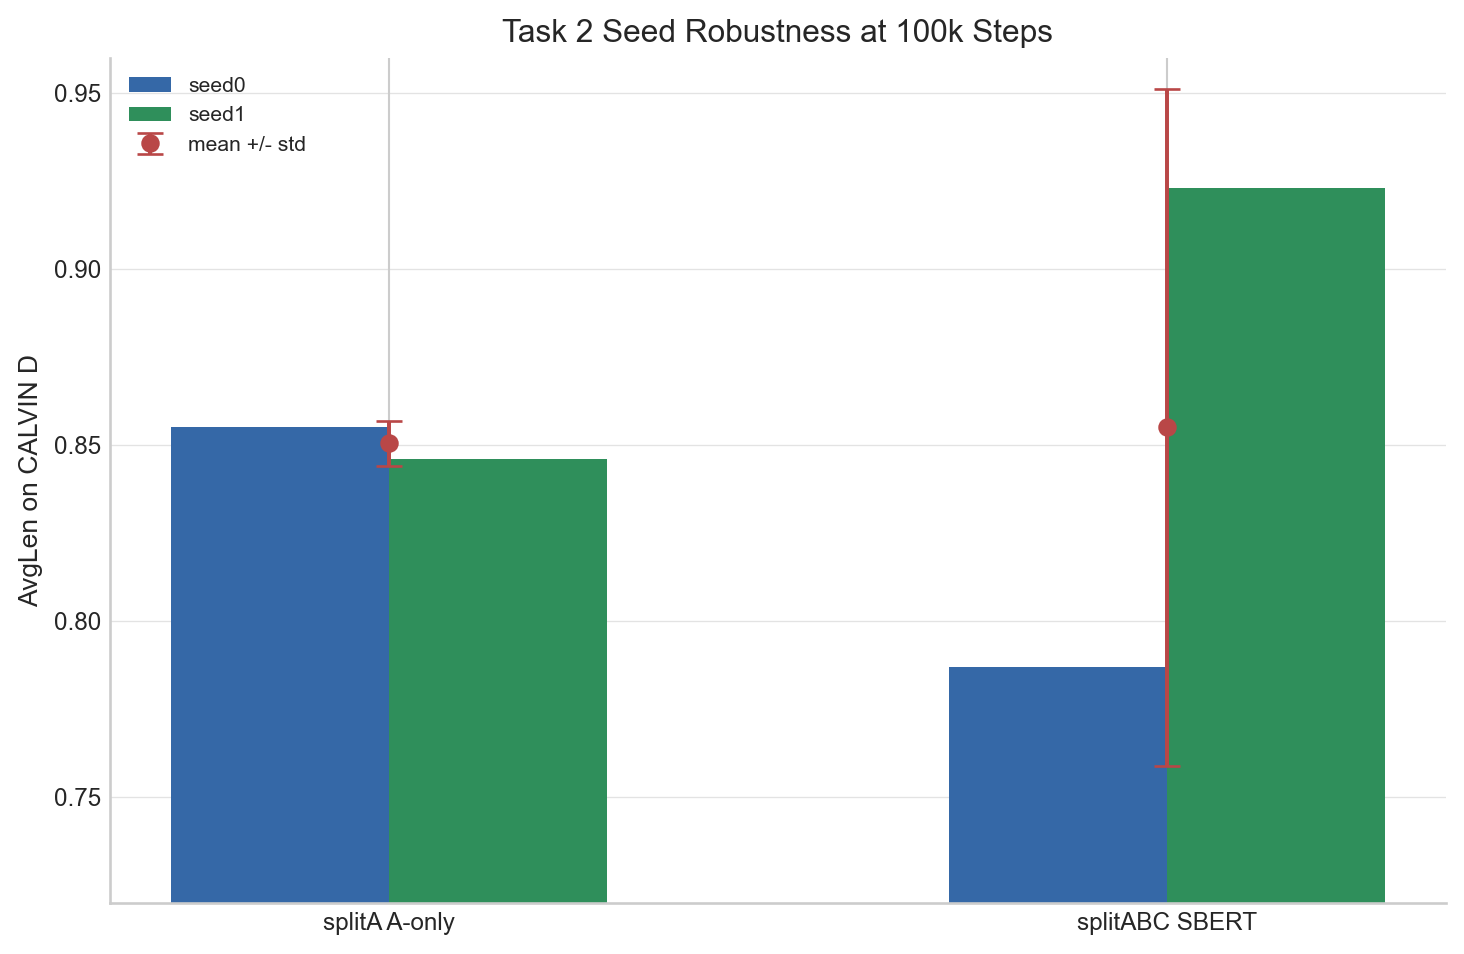
\includegraphics[width=0.76\textwidth]{task2_seed_robustness.png}
    \caption{课程显式 split 上 A-only 与 ABC SBERT 的 seed 稳健性}
    \label{fig:task2-seed-robustness}
\end{figure}

\begin{figure}[!htbp]
    \centering
    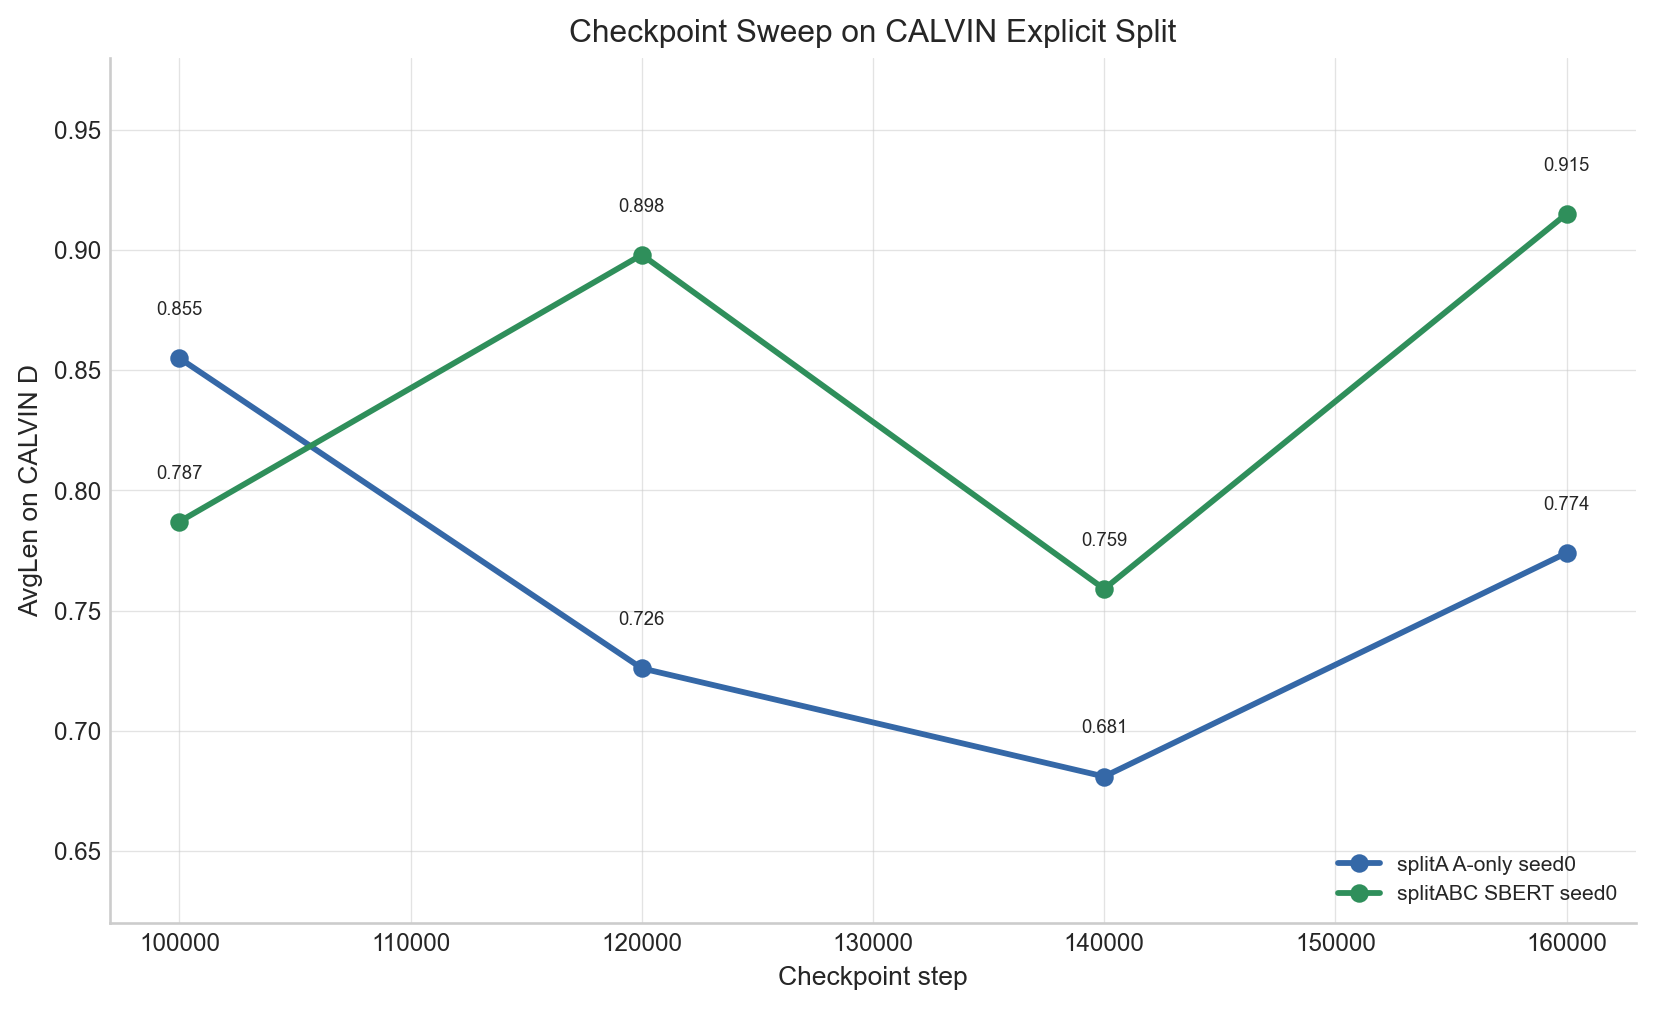
\includegraphics[width=0.92\textwidth]{task2_checkpoint_sweep.png}
    \caption{课程显式 split 上 checkpoint sweep 的 Avg Len 变化}
    \label{fig:task2-checkpoint-sweep}
\end{figure}

图~\ref{fig:task2-seed-robustness} 和图~\ref{fig:task2-checkpoint-sweep} 显示，A-only 的均值和方差更稳定；ABC SBERT 的均值略高、方差更大，因此多环境策略需要同时报告 seed 和 checkpoint。ABC SBERT seed0 在更长训练后提升到 0.915，说明语言语义条件在足够训练和合适 checkpoint 下能够缓解直接混合 A/B/C one-hot 数据带来的干扰。

\subsection{ACT 动作分块机制}

ACT 的核心机制是一次预测未来动作片段，而不是每一步只输出一个动作。动作分块长度会同时影响动作平滑性和闭环纠错频率：chunk 太短时策略更频繁地重新规划，容易放大视觉扰动；chunk 太长时动作片段更完整，但错误也可能持续更久。表~\ref{tab:act-extensions} 汇总了 chunk size、任务条件和训练时长相关实验。

\begin{table}[!htbp]
    \centering
    \caption{ACT 扩展实验在 CALVIN D 上的结果}
    \label{tab:act-extensions}
    \small
    \begin{tabularx}{\textwidth}{Xrrrr}
        \toprule
        配置 & Condition & Avg Len & SR@1 & SR@5 \\
        \midrule
        Unconditioned ACT & none & 0.097 & 0.094 & 0.000 \\
        Task-conditioned ACT & one-hot & 0.671 & 0.411 & 0.006 \\
        Language-conditioned ACT & SBERT & 0.688 & 0.434 & 0.009 \\
        Language-conditioned ACT & hash & 0.492 & 0.373 & 0.001 \\
        Task-conditioned, chunk 10 & one-hot & 0.523 & 0.323 & 0.007 \\
        Task-conditioned, chunk 100 & one-hot & 0.791 & 0.517 & 0.004 \\
        Task-conditioned, wrong one-hot & wrong & 0.076 & 0.075 & 0.000 \\
        Task-conditioned, zero one-hot & zero & 0.034 & 0.033 & 0.000 \\
        ABC extended 200k ckpt120k & one-hot & 1.028 & 0.561 & 0.022 \\
        splitABC SBERT 100k & SBERT & 0.787 & 0.477 & 0.012 \\
        splitABC chunk100 100k & one-hot & 0.696 & 0.457 & 0.008 \\
        splitABC SBERT seed1 100k & SBERT & 0.923 & 0.496 & 0.021 \\
        splitABC SBERT seed0 160k & SBERT & 0.915 & 0.483 & 0.022 \\
        splitA A-only seed1 100k & one-hot & 0.846 & 0.487 & 0.011 \\
        splitA A-only seed0 160k & one-hot & 0.774 & 0.482 & 0.009 \\
        \bottomrule
    \end{tabularx}
\end{table}

动作分块实验显示，chunk size 对跨环境泛化有明显影响。ABC 扩展训练数据上，chunk 10 的 Avg Len 为 0.523；chunk 100 的 Avg Len 为 0.791，SR@1 达到 0.517。显式 split 上的 splitABC chunk100 得到 Avg Len 0.696，同 split 的 SBERT 条件模型得到 0.787。checkpoint sweep 显示，默认 chunk 50 配合 SBERT 条件和合适 checkpoint 是当前结果中更有效的组合：SBERT seed1 100000 step 和 seed0 160000 step 分别达到 0.923 和 0.915。因此，Action Chunking 的作用主要体现在短序列成功率、动作平滑性和误差传播方式之间的平衡。

任务条件消融进一步说明，ACT 在 CALVIN 多任务数据中需要明确的任务目标。未使用 task condition 的模型在 D 上 Avg Len 只有 0.097；错误 one-hot 和零 one-hot 的结果也明显偏低。相比之下，正常 one-hot、SBERT 条件和经过 checkpoint 选择的 SBERT 模型均有更高在线表现，说明条件输入不是附加装饰，而是策略区分不同任务动作意图的必要信息。

\subsection{视觉分布偏移分析}

Visual Distribution Shift 分析关注训练环境与 D 测试环境在图像观测上的差异，以及这种差异是否能直接解释 zero-shot 成功率。表~\ref{tab:task2-shift} 给出了不同数据划分与环境 D 之间的视觉距离，并同时统计动作序列平滑性。RGB L2 越低表示与 D 的平均视觉差异越小；Mean action delta 和 P95 action delta 描述相邻动作变化幅度。

\begin{table}[!htbp]
    \centering
    \caption{Visual distribution shift 与动作平滑性统计}
    \label{tab:task2-shift}
    \small
    \begin{tabular}{lrrrr}
        \toprule
        数据划分 & RGB L2 top$\to$D & RGB L2 wrist$\to$D & Mean action delta & P95 action delta \\
        \midrule
        A & 0.0288 & 0.0262 & 0.2260 & 0.5671 \\
        B & 0.0263 & 0.0267 & 0.2257 & 0.5665 \\
        C & 0.0199 & 0.0270 & 0.2237 & 0.5599 \\
        ABC & 0.0250 & 0.0265 & 0.2251 & 0.5646 \\
        \bottomrule
    \end{tabular}
\end{table}

\begin{figure}[!htbp]
    \centering
    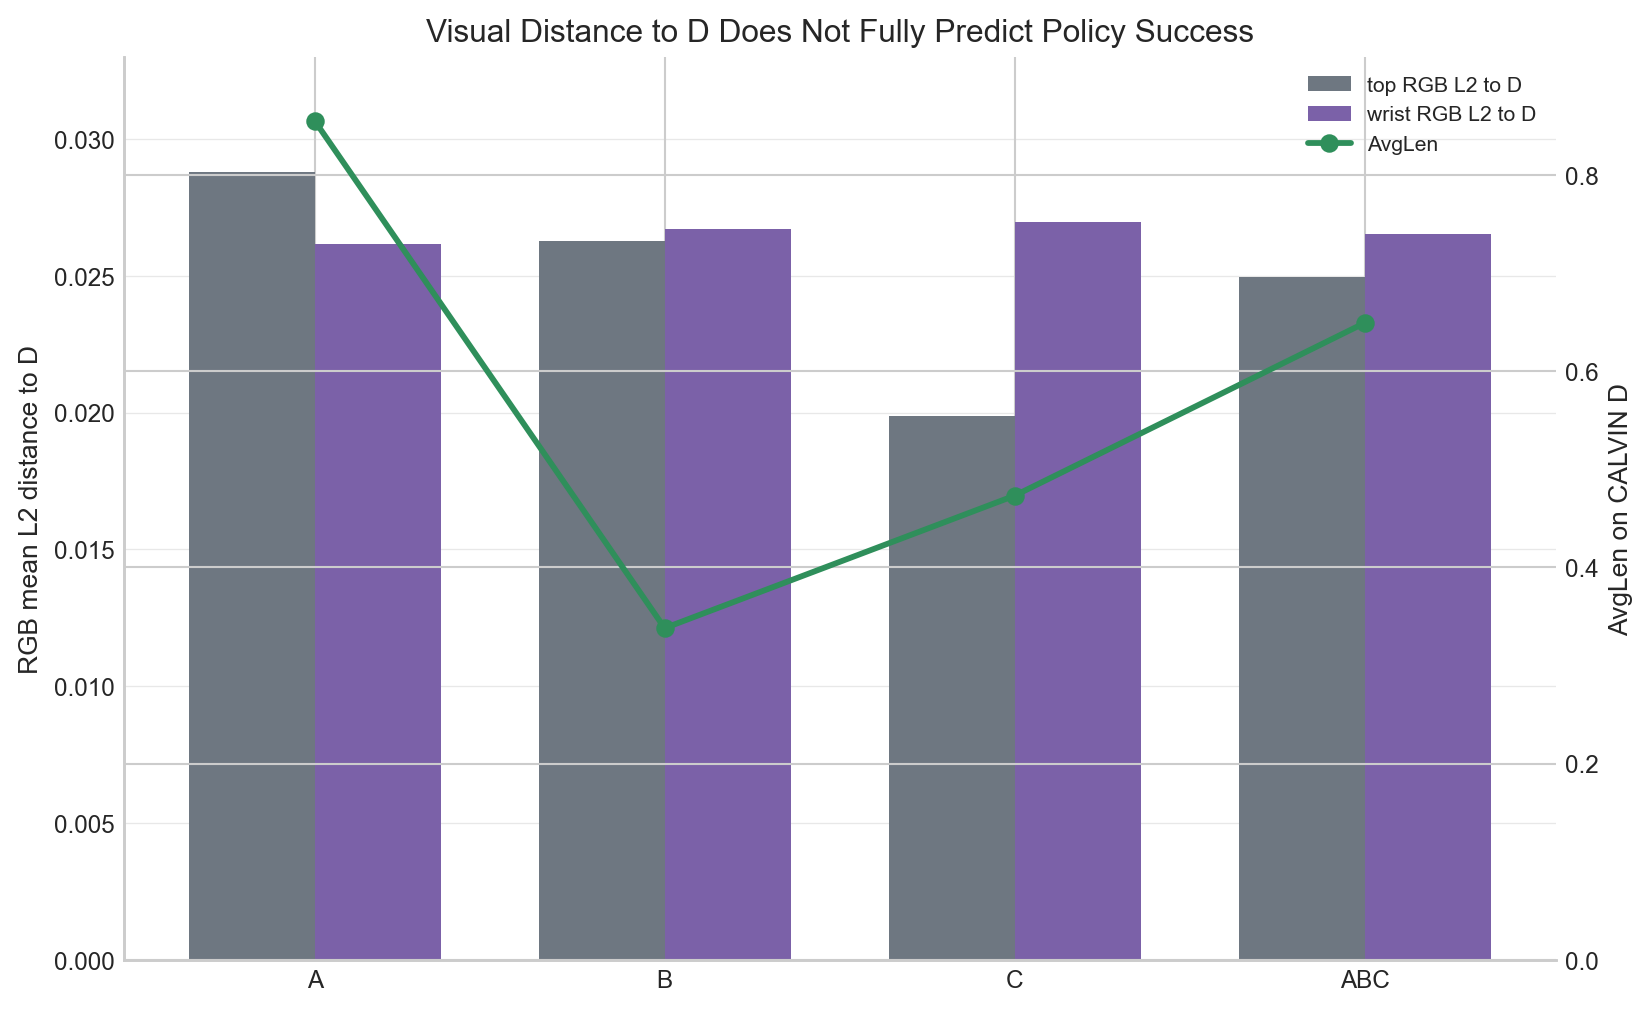
\includegraphics[width=0.84\textwidth]{task2_visual_action_shift.png}
    \caption{训练 split 到环境 D 的视觉距离与动作平滑性}
    \label{fig:task2-visual-action-shift}
\end{figure}

从视觉统计看，C 段的 top-view RGB 距离 D 最近；但在显式 split 单环境训练中，C-only 的 Avg Len 为 0.473，A-only 为 0.855。这说明平均视觉距离只是策略泛化的一个因素，不能单独解释在线成功率。任务覆盖、动作分布、局部交互状态以及训练数据多样性都会影响 D 环境表现。ABC-mixed 整合了更多环境变化；ABC 扩展训练的长训练和 checkpoint sweep 结果更高，说明数据规模、任务覆盖、训练时长和 checkpoint 选择仍然是影响性能的重要因素。

图~\ref{fig:task2-visual-action-shift} 显示同样趋势：C 的 top-view RGB 距离最小，但 wrist-view 距离并不最小，且单环境策略表现还受到动作先验和任务覆盖影响。这说明 CALVIN 策略泛化需要结合腕部相机、机器人状态、动作先验和任务语义共同分析。

\begin{figure}[!htbp]
    \centering
    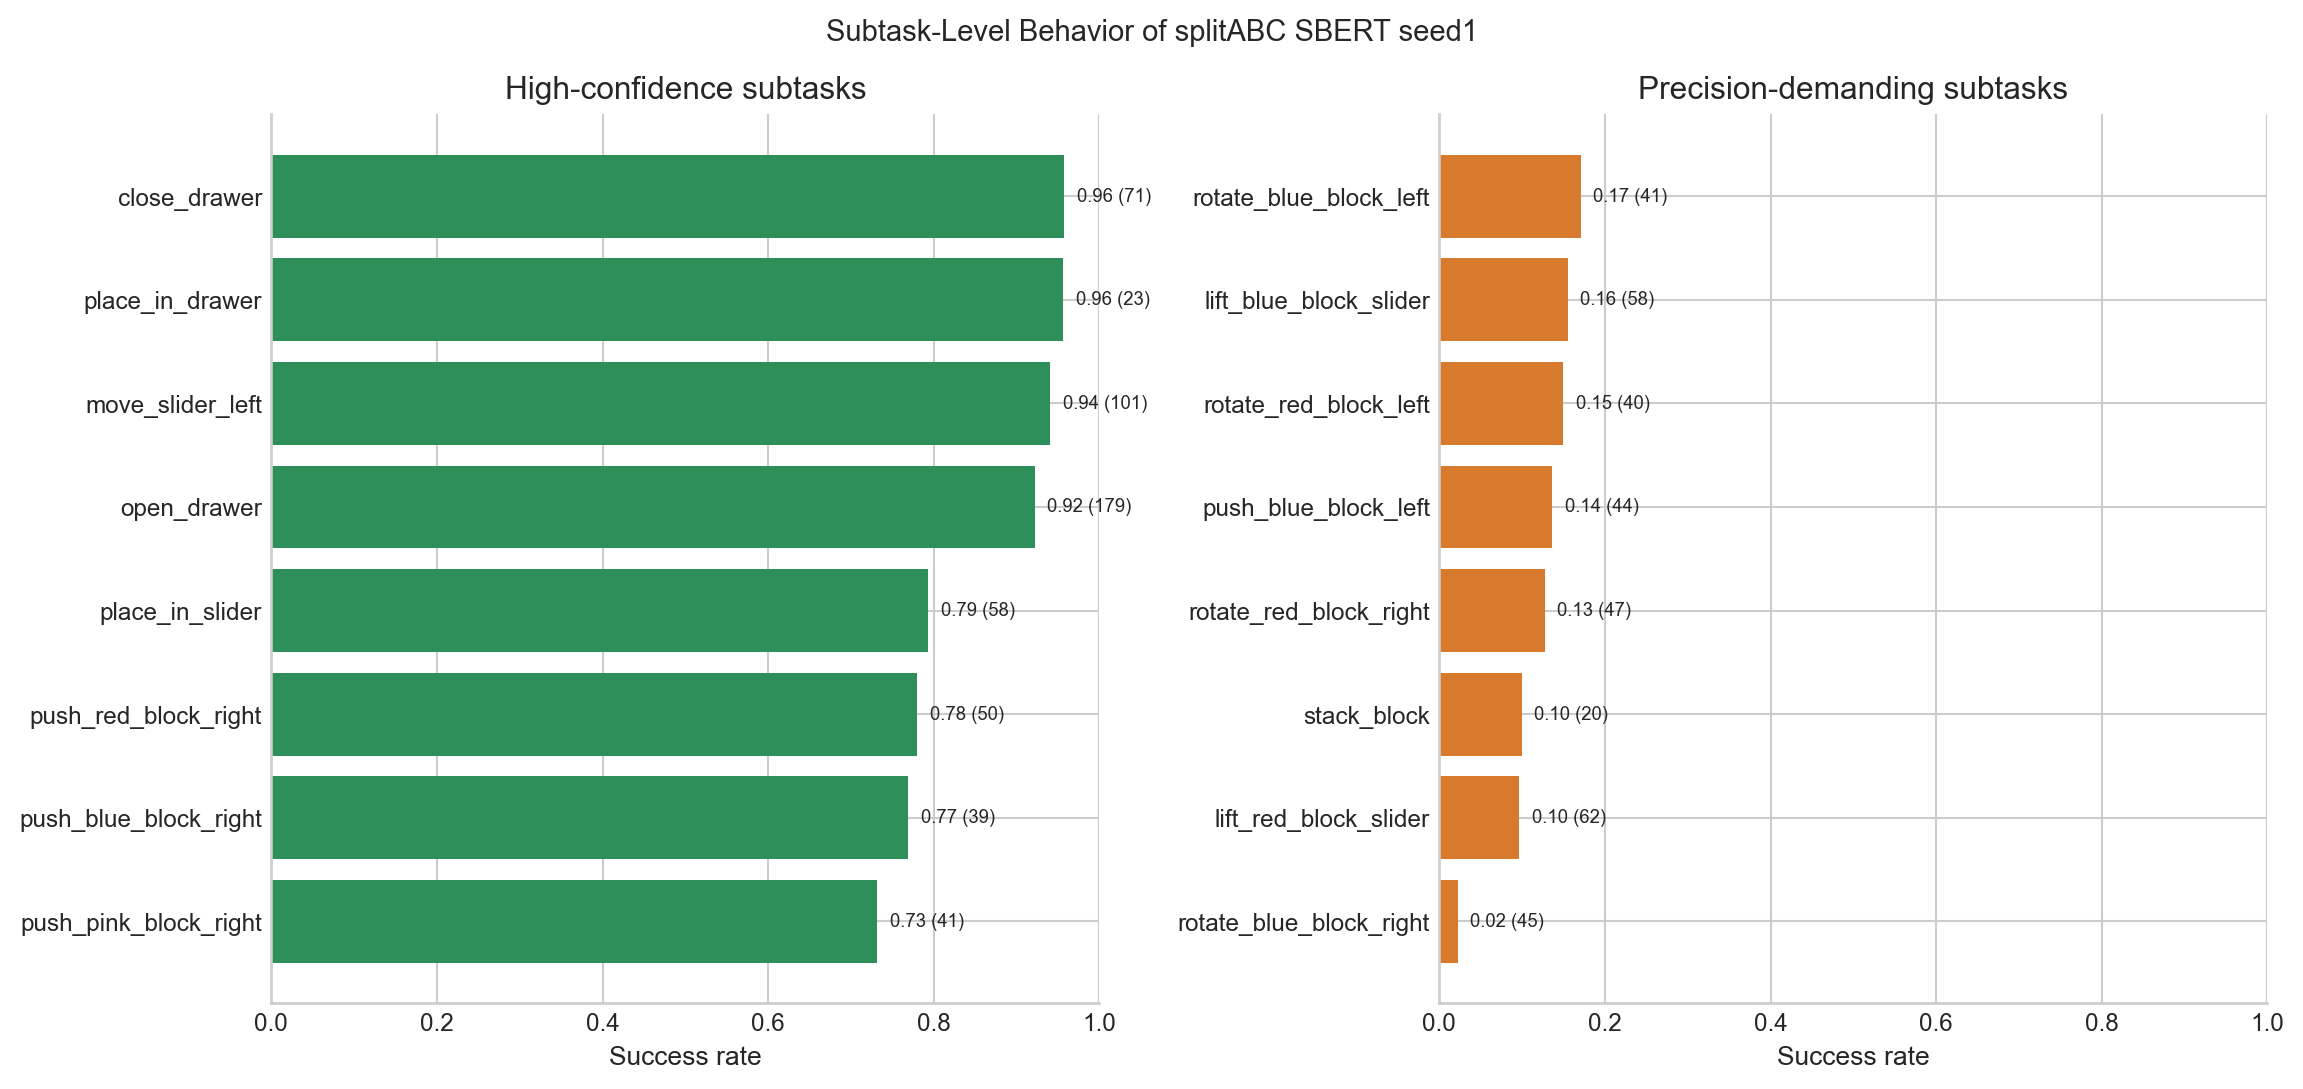
\includegraphics[width=0.86\textwidth]{task2_subtask_breakdown.png}
    \caption{splitABC SBERT seed1 最终策略的子任务行为分解}
    \label{fig:task2-subtask-breakdown}
\end{figure}

在视觉偏移之外，长任务链还受不同子任务难度影响。本文进一步解析 splitABC SBERT seed1 的评测明细。图~\ref{fig:task2-subtask-breakdown} 显示，抽屉开合、放入抽屉和滑块移动类动作成功率较高；积木旋转、从滑块处取放物体和堆叠类动作对接触、姿态调整和连续纠错要求更高。该分析解释了为什么整体 Avg Len 能接近 1，而 SR@3--SR@5 更依赖长链任务中的精细接触控制。

\section{结论}

本文完成题目一的三类物体构建、Mip-NeRF 360 场景重建和 A/B/C 场景融合。物体 A 使用 73 张手机多视角图像完成 COLMAP+3DGS 重建，得到 5293 个 COLMAP 稀疏点和 146445 个 Gaussian centers；物体 B、C 分别由 threestudio text-to-3D 和 Zero123 image-to-3D 生成。三个 Mip-NeRF 360 场景均完成 3DGS 训练与定量评价，其中 \code{counter} 主实验达到 PSNR 29.6144、SSIM 0.9290、LPIPS 0.1007。最终融合阶段将 A/B/C 与 \code{counter} 背景统一转换或导入为 mesh，在 Blender 中完成材质、坐标和相机轨迹设置，并导出 150 帧漫游视频。

题目二完成 LeRobot ACT 的基础策略训练、混合策略训练和 D 环境 zero-shot 测试。splitA A-only 在 100000 step 达到 Avg Len 0.855，splitABC one-hot、SBERT 和 chunk100 分别为 0.649、0.787 和 0.696；seed 与 checkpoint 实验中，splitABC SBERT seed1 100000 step 达到 0.923，seed0 160000 step 达到 0.915，ABC 扩展训练在 120000 step checkpoint 达到最佳 Avg Len 1.028。结果表明，任务条件表达、ACT 动作分块、训练时长和 checkpoint 选择共同影响 D 环境泛化；视觉距离和子任务分解也说明，zero-shot 控制需要同时考虑视觉分布与长链误差传播。

\end{document}
